
\chapter{Translocation avec membrane fixe}
\label{translocmurfixe}
\cleardoublepage
{\Large\textbf{Translocation avec membrane fixe}
}\\

\lettrine[loversize=0.6,lraise=0.1,findent=0.5em,nindent=0em]{D}{}ans ce chapitre, nous discutons dans un premier temps des préliminaires afin d'aborder la translocation. Après avoir défini la membrane et les conditions d'équilibration précédent la translocation, nous présentons les différentes théories de la translocation non biaisée puis de la translocation forcée et terminons sur les distributions de temps de translocation attendues. Dans un second temps, nous testons notre polymère dans le cas simple de la translocation à travers une membrane fixe. Cette deuxième partie permet de comparer polymère linéaire simple et polymère structuré ainsi que pore large et pore étroit. Nous proposons également un modèle théorique permettant d'expliquer les différentes phases de la translocation biaisée par l'application d'une force en bout de chaîne et de déterminer le temps de translocation.\\

\minitoc

\begin{center}
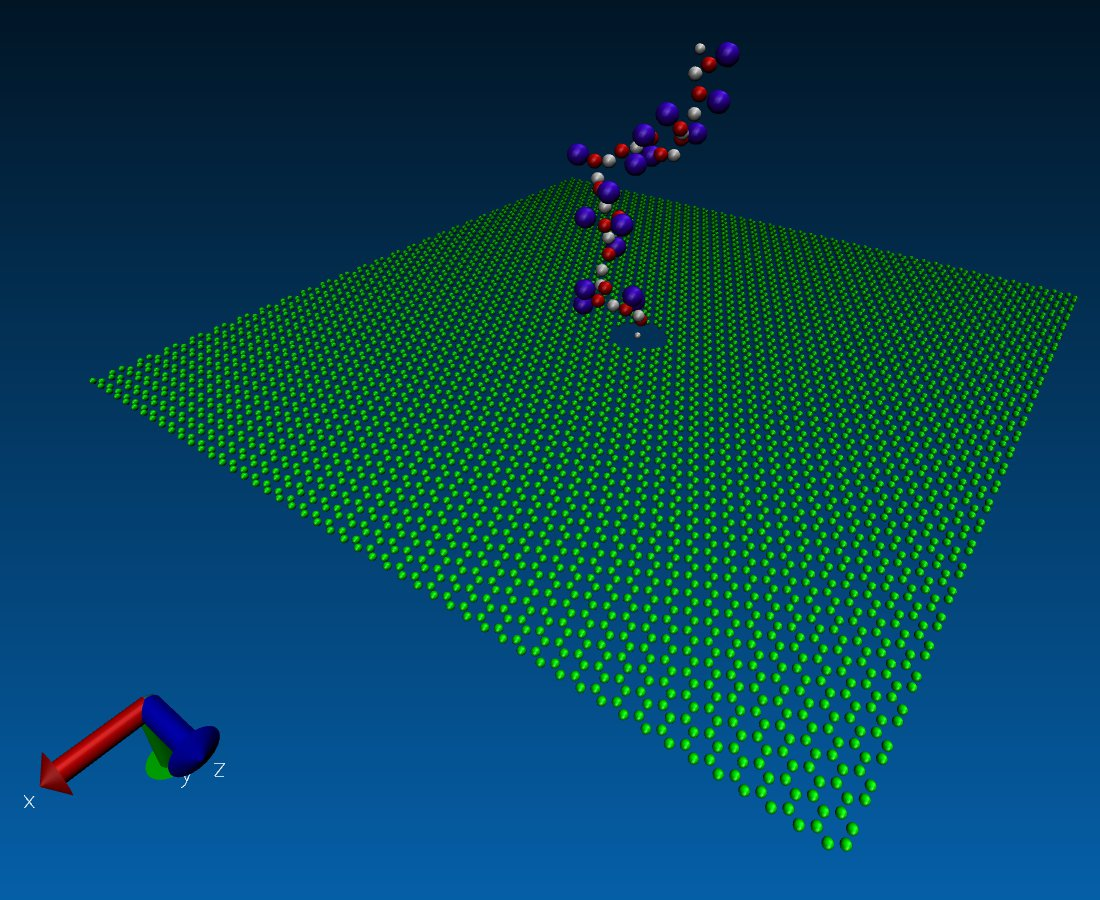
\includegraphics[width=0.7\textwidth]{confinit.jpg}
\end{center}



\cleardoublepage








\section{Préparation à la translocation}

\subsection{Définition de la membrane}

Bien que d'autres cristaux bidimensionnels existent, le graphène reste le candidat principal pour le séquençage en utilisant des nanopores dans des membranes fines. Nous avons donc considéré un modèle de membrane proche de ce dernier.
Afin de modéliser la membrane à travers laquelle notre polymère va effectuer une translocation, nous avons choisi de respecter les dimensions relatives  entre le graphène et l'ADN. Un réseau hexagonal de paramètre de maille $\frac{\sigma}{2}$ a été généré (voir figure \ref{reseau}). Le plan de graphène est suffisamment étendu pour qu'avec des conditions aux limites périodiques (pour simuler un plan infini), le polymère le plus grand utilisé ne puisse jamais se retoucher lui même, soit 5488 grains. Cette étendue importante implique que les atomes de notre membrane seront les atomes majoritaires.

\begin{figure}[H]
\begin{center}
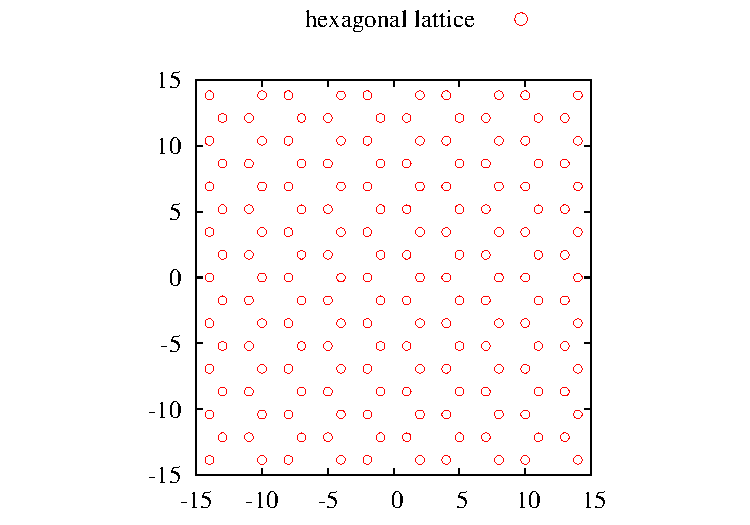
\includegraphics[width=0.65\textwidth]{lattice.pdf} 

\caption{Réseau héxagonal constituant la membrane}
\label{reseau}
\end{center}
\end{figure}

Le réseau est ensuite amputé en son centre de tous les grains situés dans un rayon fixé pour créer le pore. Dans ce chapitre, les grains de la membrane sont fixes, les équations du mouvement ne sont pas intégrées pour la membrane, elle n'existe qu'à travers l’Interaction avec le polymère par des potentiels stériques de type Lennard-Jones. Afin d'éviter que le polymère ne pénètre entre les grains de notre membrane, nous avons choisi $\sigma_{ij}=\sigma$ pour toute interaction avec un grain de la chaîne du polymère et $\sigma_{ij}=1.25\sigma$ pour un grain latéral. Cette valeur est supérieur à l'espacement entre grains de la membrane. Physiquement, dans le cas du graphène ces tailles correspondent à la taille des orbitales atomiques de type $\pi$ du graphène avec lesquelles le polymère interagit.


\subsection{Polymère greffé et configurations initiales}

Dans un premier temps, rappelons comme nous l'avons décrit dans le \hyperref[intro]{chapitre 1} que la translocation peut se dérouler dans différents contextes. Elle peut être due uniquement aux fluctuations thermiques, on parle alors de translocation non biaisée, ou être pilotée par une force extérieure, on parle alors de translocation forcée (driven translocation). Les forces extérieures peuvent être de natures variées, on citera notamment l'utilisation de champs électriques (électro- phorèse), de gradients de potentiels chimiques, de flux imposé sur le solvant, ou encore l'emploi de pinces (optiques ou magnétiques) \cite{keyser}. Nous avons choisis de nous placer dans ce dernier cas, notre polymère est donc tracté par une de ses extrémités. En effet, l'alternative plus courante d'appliquer une force au centre du pore (ce qui représente un gradient de potentiel chimique ou électrique) impose de définir une zone d'application de la force qui est clairement définie dans les modèles simples, mais qui deviendrait vite compliquée dans les cas de déformation de la membrane, comme nous l'envisagerons au \hyperref[chapitrememflex]{chapitre 4}. Puisque nous souhaitons que les conditions soient comparables, nous opterons pour la traction de notre polymère en bout de chaîne.



Nous avons dans le \hyperref[intro]{chapitre 1} parlé d'une barrière d'énergie à franchir pour effectuer la translocation d'un polymère, calculons la. Pour cela, nous devons dans un premier temps détermi- ner la probabilité de distribution d'un polymère idéal greffé à une paroi. La chaîne idéale présente comme conditions aux limites, la non pénétration des monomères à travers la paroi. On note $P(\textbf{r},\textbf{r}_0,n)$ la probabilité de trouver le $n$-ième monomère en position $\textbf{r}$, pour $n \gg 1$, le premier monomère étant greffé en $\textbf{r}_0$. $P_0$ est la distribution calculée dans le \hyperref[eqdif]{chapitre précédent} pour un polymère idéal libre:

\begin{eqnarray}
P_0(\textbf{r},\textbf{r}_0,n)=\left(\frac{3}{2\pi n b^2}\right)^\frac{3}{2}\exp\left(-\frac{3(\textbf{r}-\textbf{r}_0)^2}{2 n b^2}\right)
\end{eqnarray}

A l'instar de nombreux problèmes d'électromagnétisme ou de mécanique des fluides, on utilise la méthode des images miroirs afin de déterminer $P(\textbf{r},\textbf{r}_0,n)$. En effet, on a:

\begin{eqnarray}
P(\textbf{r},\textbf{r}_0,n) \propto P_0(\textbf{r},\textbf{r}_0,n)-P_0(\textbf{r},-\textbf{r}_0,n)
\end{eqnarray}

La membrane joue alors le rôle de miroir plan (analogie optique \cite{lipson2011optical}), de conducteur (analogie électrostatique \cite{jackson1999classical}) ou encore d'obstacle sur lequel rebondi un jet (source miroir en mécanique des fluides \cite{kundu2008fluid}).

Dans le cas idéal, la probabilité de distribution du monomère de queue est à variables séparables. En posant $\textbf{r}_0= \epsilon y$ avec $\epsilon \ll 1$, un développement limité au premier ordre donne:

\begin{eqnarray}
P(\textbf{r},\textbf{r}_0,n) \propto \left(\frac{3}{2\pi n b^2}\right)^\frac{3}{2} \left(\frac{6 y \epsilon}{n b^2}\right)\exp\left(-\frac{3\textbf{r}^2}{2 n b^2}\right)
\end{eqnarray}

Cette probabilité est à variables séparables, c'est à dire qu'elle peut s'écrire comme le produit d'une fonction de x, d'une fonction de y  et d'une fonction de z. Selon x et z (la membrane occupant le plan y=0), la distribution reste inchangée (et donc gaussienne) par rapport au cas du polymère libre, il n'y a une influence sur les configurations interdites par la membrane que selon l'axe y. Pour le cas d'un polymère non idéal, les termes supplémentaires introduits dans $P_0$ ne permettent pas de séparer les variables et d'obtenir une expression analytique. Cependant l'allure de la distribution du monomère de queue reste proche du cas idéal tout en présentant des caractéristiques dues aux volumes exclus (voir figure \ref{polagainstwall}). Afin d'aborder la translocation, nous avons dû créer des configurations indépendantes de polymères à l'équilibre, juste avant l'application d'une force. Lors de ce processus de génération, nous avons laissé le polymère évoluer librement en fixant une extrémité au centre du pore. Les 1000 configurations initiales sont toutes séparées d'au moins dix temps de corrélation du polymère afin de garantir qu'elles soient statistiquement indépendantes.


\begin{figure}[H]
\begin{center}


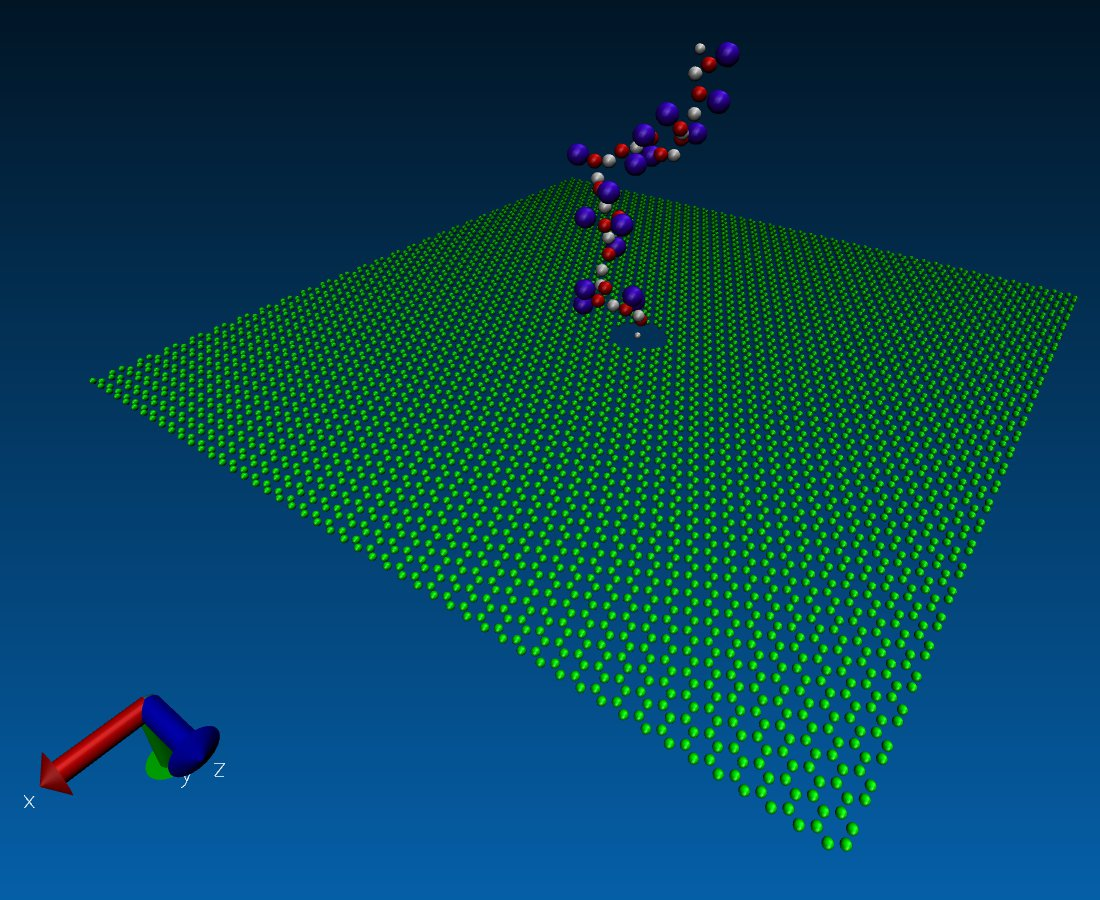
\includegraphics[width=0.7\textwidth]{confinit.jpg}
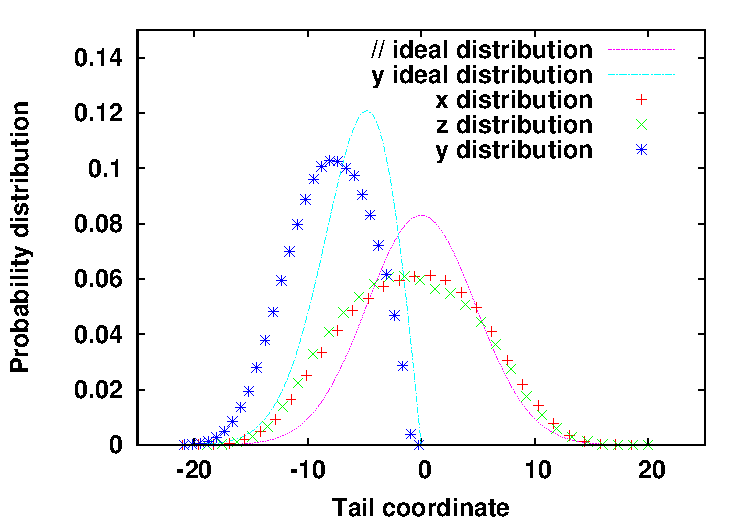
\includegraphics[width=0.9\textwidth]{probdistribution.pdf}


\caption[Polymère greffé sur une membrane]{En haut: Capture d'écran de la visualisation avec VMD \cite{HUMP96,STON2001} d'une configuration de notre polymère structuré évoluant avec une extrémité fixée au centre du nano-pore. En bas, probabilité de distribution théorique du monomère de queue pour un polymère idéal et résultats numériques pour notre polymère (N=35 grains latéraux). Parallèlement à la membrane, la distribution gaussienne idéale est aplatie au centre à cause de la zone d'exclusion des autres monomères. De même pour la direction perpendiculaire, le pic maximum est repoussé par la présence d'autres monomères. Dans les deux cas, l'éloignement maximal n'est pas modifié car le cas idéal correspond déjà à des chaînes étirées sans superposition de monomères. }
\label{polagainstwall}
\end{center}
\end{figure}

\section{Théories de la translocation}

\subsection{Théories de la translocation non biaisée}


La probabilité de distribution du polymère accolé à une membrane permet, à partir de la fonction de partition stérique, $Z_S(n)= \int_{y>0} P(\textbf{r},\textbf{r}_0,n) \textbf{dr}$, de calculer l'énergie libre d'origine entropique d'un tel système. Dans la limite $n \gg 1$, le premier terme non nul du développement limité impose la loi d'échelle: $Z_S(n) \propto n^{\gamma'-1}$ (on aura un facteur $\gamma'$=1/2 pour un polymère gaussien, 0.68 pour un polymère avec volumes exclus,  ($\nu$=0.588) ou 1 pour une chaîne rigide). Pour un polymère idéal de $N$ monomères en cours de translocation, lors du passage du $n$-ième monomère, Sung et Park \cite{Sung1996} décrivirent les premiers la valeur de l'énergie libre en prenant en compte les effets entropiques de part et d'autre de la membrane:
\begin{eqnarray}
F(N,n)= -k_BT\ln\left(Z_S(n)Z_S(N-n)\right)= \frac{1}{2} k_BT \ln \left(n(N-n)\right) +cste
\label{energbar}
\end{eqnarray}

Cette barrière d'énergie à franchir au cours de la translocation peut être altérée en appliquant une différence de potentiel, chimique ou électrique, ou encore en appliquant directement une force sur la chaîne. La Figure \ref{energiebarrier} montre cette barrière d'énergie.
 Dans le cas d'un polymère non idéal avec volumes exclus, Muthukumar \cite{Muthukumar1999} a montré que l'équation du polymère idéal \ref{energbar} était une simplification de l'équation suivante plus générale:

\begin{eqnarray}
\frac{F(N,n)}{k_BT}= (1-\gamma_2')\ln(n)+ (1-\gamma_1')\ln(N-n)+cste
\label{energbarsaw}
\end{eqnarray}

avec $\gamma_i'$ l'exposant caractéristique de la taille du polymère dans le milieu i ($\gamma_i'$=0.5 pour un polymère idéal ou un milieu saturé en polymère,$\gamma_i'$=0.68  pour un polymère avec volumes exclus ($\nu$=0.588) ou encore 1 pour des polymères ultra rigides ou rod-like en anglais).

Dans le cas général, $\gamma_1'$=$\gamma_2'$ et la translocation est biaisée par une différence de potentiel (chimique, électrique...), on alors la relation:

\begin{eqnarray}
F(N,n)= -k_BT(1-\gamma')\ln \left(n(N-n)\right) + n \Delta \mu +cste
\label{energbargen}
\end{eqnarray}

Dans notre cas, nous n'avons pas une différence d'énergie qui s'applique à la barrière entropique, mais la contribution du travail d'une force (sa transmission le long de la chaîne sera discutée avec les résultats).

Sung, Park et Muthukumar \cite{Sung1996,Muthukumar1999} utilisent cette énergie pour résoudre l'équation dite de Fokker-Planck qui traite l'évolution de la probabilité d'avoir $n$ monomères qui ont effectué la translocation:
\begin{eqnarray}
\frac{\partial P(n,t)}{\partial t} =   \mathcal{L}_{FP}(n) P(n,t)
\label{equfokkerplank1}
\end{eqnarray}

Avec l'opérateur $\mathcal{L}_{FP}(n)= (1/b^2)(\partial/\partial n) D(n)[\exp(-F(N,n)/k_BT)](\partial/\partial n)[\exp(F(N,n)/k_BT)]$

Chuang, Kantor et Kardar \cite{Chuang2001} notèrent que cette équation, dans le cas non biaisé, peut être réduite à:

\begin{eqnarray}
\frac{\partial P(n,t)}{\partial t} =   \frac{\partial ^2 P(n,t)}{\partial ^2 n} +(1-\gamma') \frac{\partial  }{\partial  n}\left(P(n,t)\frac{1-2n}{(1-n)n}\right)
\label{equfokkerplank2}
\end{eqnarray}
grace aux changements de variable:
$n \rightarrow nN$ et $t \rightarrow tD/N^2$


Gardons à l'esprit que ces équations sont valables dans la mesure où le polymère demeure à l'équilibre thermodynamique au cours de la translocation, hypothèse de travail qui sera remise en cause par la suite.



\begin{figure}[H]
\begin{center}
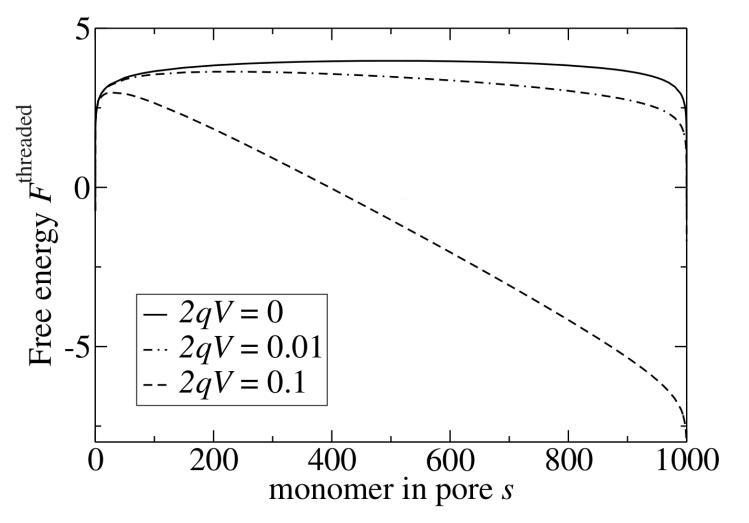
\includegraphics[width=0.7\textwidth]{transelec.jpg} 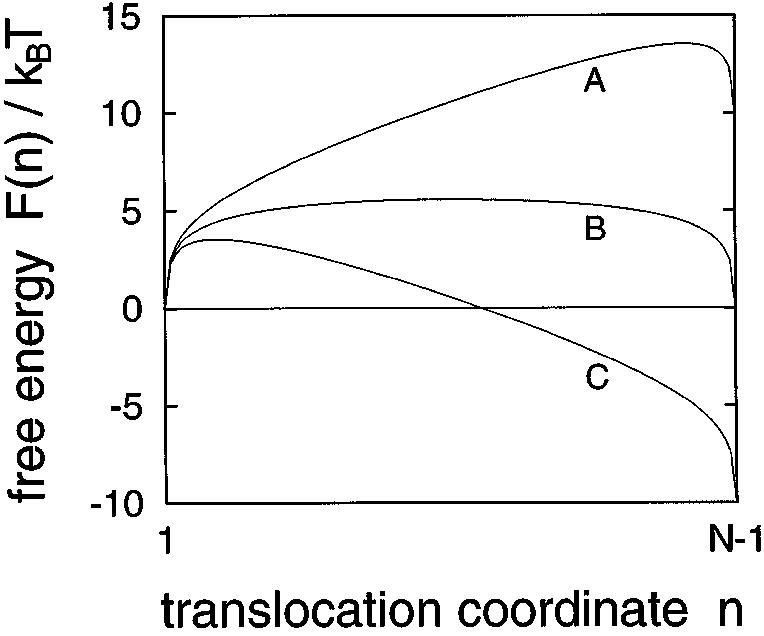
\includegraphics[width=0.5\textwidth]{transpotchim.jpg}

\caption[Translocation, barrière d'énergie d'origine entropique]{Modification de la barrière entropique par une différence de potentiel électrique (en haut \cite{these}) et de potentiel chimique (en bas \cite{Sung1996}). A: différence de potentiel opposée à la translocation, B: différence de potentiel nulle, C: différence de potentiel favorable.}
\label{energiebarrier}
\end{center}
\end{figure}

L'équation précédente \ref{equfokkerplank2} ne faisant plus apparaître $N$, on peut en déduire qu'il existe un paramètre $\alpha$ universel qui permet de décrire le temps de translocation.
\begin{eqnarray}
\tau \propto N^\alpha
\label{tauunbiased}
\end{eqnarray}


 Reste à déterminer $\alpha$. En utilisant des conditions aux limites appropriées (réfléchissante en 0 pour empêcher le retour du polymère et absorbante en bout de chaîne) la résolution de l'équation de Fokker-Planck donne $\tau \propto N^{2}/D$. Le coefficient de diffusion à utiliser est sujet de discorde, Sung et Park \cite{Sung1996} considèrent le coefficient de diffusion comme étant celui du polymère libre et donc inversement proportionnel à $N$ (\hyperref[fluctudissip]{voir chapitre 2}), ce qui leur fait prédire $\tau \propto N^{3}$, Muthukumar \cite{Muthukumar1999} lui, considère que c'est le coefficient de diffusion du polymère au sein du pore qui est pertinent (D est donc une constante) d'où son affirmation $\tau \propto N^{2}$.
 
  Cependant, ses exposants sont vite remis en question par Chuang, Kantor et Kardar \cite{Chuang2001}. Ils arguent que le temps de translocation ne peut pas être plus court que le temps de relaxation du polymère, proportionnel à $N^{1+2\nu}$(comme nous l'avons vu au \hyperref[fluctudissip]{chapitre 2}), qui est caractéristique d'un déplacement du polymère sur une distance de l'ordre de son rayon de giration (comme si il n'y avait pas de membrane à franchir). Si l'exposant associé au temps de translocation est plus faible que le temps de relaxation, cela voudrait dire que la chaîne n'a pas le temps de s'équilibrer au cours de la translocation et donc qu'on ne peut pas appliquer l'équation de Fokker-Planck au système. On a alors un phénomène de translocation sous-diffusif.
  
   Des essais de résolution ont été menés en utilisant une équation de Fokker-Planck fractionnelle \cite{Metzler2003} (qui s'applique dans un cas plus général) et trouvent $\tau \propto N^{2+2\nu-\gamma'}$. Une approche suggère une translocation avec plusieurs échelles de temps représentant l'équilibration des liaisons et la diffusion, on aurait alors $\tau \propto N^{2+\nu}$. Une autre tentative d'approche théorique est à partir de l'équation de Langevin généralisée \cite{Panja2010} et prédit $\tau \propto N^2$ pour un polymère idéal, $\tau \propto N^{2+\nu}$ dans le cas de Rouse et $\tau \propto N^{1+2\nu}$ dans le cas de Zimm (avec interactions hydrodynamiques). Il est intéressant de noter que Luo et al. \cite{2Luo2006} trouvent une évolution de $\alpha=1+2\nu$ à $\alpha=1$ lorsque la longueur du pore augmente.
   
   Les simulations numériques effectuées n'apportent pas de consensus et estiment des exposants compris entre 2.2 et 2.6, suggérant une forte dépendance aux conditions de simulation et une possibilité d'existence de différent régimes en fonction de l'importance de la friction. En effet une transition entre les deux exposants $1+2\nu$ et $2+\nu$ a été reportée \cite{Panja22010}. Le lecteur intéressé pourra trouver un tableau récapitulatif des valeures de $\alpha$ obtenues lors de la translocation non biaisée dans l'article de revue de Palyulin, Ala-Nissila et Metzler \cite{Palyulin2014}.\\

\subsection{Théories de la translocation forcée}

La question de la translocation non biaisée qui ne fait pas consensus n'a pas empêché la communauté scientifique d'aborder le cas de l'introduction d'une force pour faciliter le phénomène. Il vient naturellement à l'esprit que la contribution d'une force appliquée vers le côté trans va favoriser la translocation et on s'attend donc à pouvoir décrire le temps de translocation de la manière suivante, toujours avec un paramètre $\alpha$ caractéristique du nombre de monomères et un nouvel exposant critique $\delta$ pour la force:

\begin{eqnarray}
\tau \propto N^\alpha / f^\delta
\label{taubiased}
\end{eqnarray}

Il est évident que l'amplitude de la force va influer sur la valeur des exposants critiques $\alpha$ et $\delta$. Dans le cas d'une force extrêmement faible, on s'attend à se retrouver dans le cas précédent de la translocation non biaisée avec $\alpha$ compris entre 2.2 et 2.6. En ce qui concerne l'autre extrême, une force très importante, la translocation est entièrement régie par la force (il n'y a plus la moindre influence de la température) et on attend $\tau \propto 1/f$.
 La plupart des études théoriques et numériques se concentrent sur le cas de l'application de la force au sein du pore. Le cas du polymère tracté est plus rarement abordé.
 
 Dans le cas général, l'hypothèse de quasi-équilibre utilisée pour résoudre analytiquement le cas de la translocation non biaisée est maintenant encore moins pertinente avec l'ajout d'une force. Il est par contre toujours possible de définir une limite inférieure à la valeur de $\alpha$. En effet si on considère le cas de l'application d'une force en l'absence de membrane, la translocation est effectuée quand le polymère a franchi une membrane virtuelle, il a donc été déplacé sur une distance de l'ordre de son rayon de giration. Or avec la friction, la vitesse moyenne du centre de masse s'écrit: $v \propto f/N$, d'où $\tau \propto N^{1+\nu}/f$. On envisage donc $\alpha=1+\nu$ comme limite inférieure \cite{Kantor2004}.
 
 Dans le cas d'une force appliquée au sein du pore, cet exposant a été tantôt confirmé tantôt infirmé. Une transition entre exposants allant de $\alpha=2\nu$ à $\alpha=1+\nu$ a vite était observée dans des modèles à deux dimensions \cite{Huopaniemi2006,2Luo2006,Luo2007}. Pour les simulations à 3 dimensions, Luo et al. \cite{Luo2009} suggèrent de distinguer la translocation lente donnant une valeur de $\alpha$ proche de $1+\nu$ trouvée par certains auteurs \cite{Kantor2004,Gauthier2008}, de la translocation rapide donnant une valeur de $\alpha$ plus faible $\alpha \approx 1.4$ \cite{Bhattacharya2009,Luo2008,Sakaue2007} (ce qui va à l'encontre de la limite inférieure proposée). Pour de faibles forces, une équation de Fokker-Planck fractionnelle en prenant en compte des effets de mémoire à longue portée \cite{Metzler2000}, un coefficient $\alpha = 1+ 2\nu - \gamma' = 1.56$ (proche $1+ \nu=1.59$) est proposé par Dubbeldam et al.\cite{Dubbeldam2007}. En utilisant la théorie de la réponse linéaire avec effets de mémoire, Vocks et al.\cite{Vocks2008} s'opposèrent aux explications de Dubbeldam et al. en proposant $\alpha= \frac{1+2\nu}{1+\nu} =1.37$. Luo et al.\cite{Luo2009} ont donc permis, comme l'illustre la figure \ref{slowandfast} de distinguer deux régimes d'application différents pour ces approches avec un phénomène fortement hors équilibre à fortes forces.
 
 
\begin{figure}[H]
\begin{center}
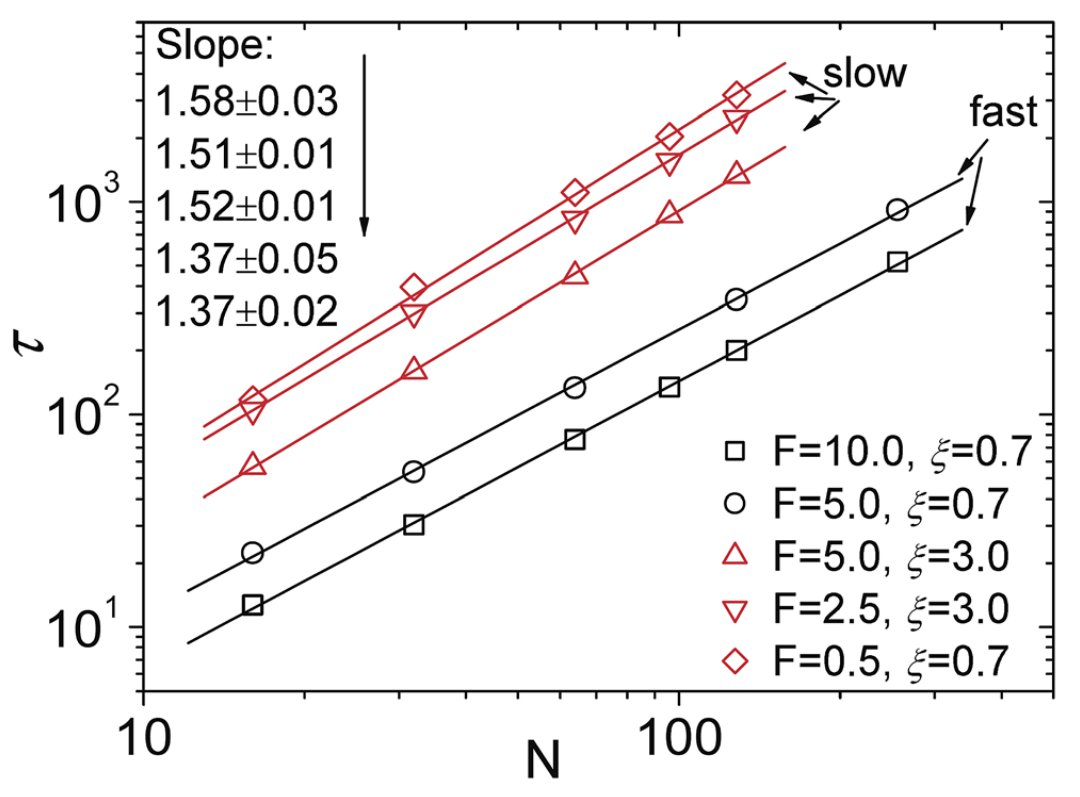
\includegraphics[width=0.9\textwidth]{slowandfasttransloc.jpg}


\caption[Translocations rapides et lentes]{Régimes proposés par Luo et al. de translocations rapides et lentes dépendants de la friction \cite{Luo2009}.}
\label{slowandfast}
\end{center}
\end{figure}

Pour la valeur de $\delta$, à force modérée, la valeur 1 ( $\tau \propto 1/f$) semble faire consensus. En revanche, à fortes forces certains auteurs trouvent un exposant modifié : $\tau \propto 1/f^{0.8}$ pour Luo et al. \cite{Luo2009} ou encore $\tau \propto 1/f^{0.95}$ pour Ikonen et al. \cite{2Ikonen2012}.

 Un tableau (\ref{tableautransloc}) résumé des différentes valeurs obtenues pour $\alpha$ et $\delta$ permet d'y voir un peu plus clairs dans les resultats et théories très variés.



\begin{table}
\setstretch{1.6}
\begin{center}


\begin{tabular}{|c|c|c|c|}
  \hline
  Valeur de $\alpha$ & Valeur de $\delta$ & Méthode & Auteur et référence \\
  \hline
  1 & \_ & 3D MC & Chern \cite{Chern2001}\\
  1 & \_  & Théorie & Lubensky \cite{Lubensky1999} \\
  1 & \_  & Expérience & Meller \cite{Meller2002} \\
  1 & 1  & 3D BD & Tian \cite{Tian2003} \\   
  1.65 $\pm$ 0.08 & \_  & 3D MC & Milchev \cite{Milchev2004} \\
  1+$\nu$, 2 (traction) & 1  & Théorie, 2D MC & Kantor \cite{Kantor2004} \\
  1+$\nu$ & \_  & Théorie & Matsuyama \cite{Matsuyama2004} \\
  1.6 & \_  & 3D MC & Tsuchiya \cite{Tsuchiya2007} \\
  1.46 $\pm$ 0.01 (courts) & \_  & 2D FB & Luo \cite{Luo2006} \\
  1.72 $\pm$ 0.06 (longs) & \_  & 2D FB & Luo \cite{Luo2006} \\
  1.50 $\pm$ 0.01 (courts) & \_  & 2D LD & Huopaniemi \cite{Huopaniemi2006} \\
  1.69 $\pm$ 0.04 (longs) & \_  & 2D LD & Huopaniemi \cite{Huopaniemi2006} \\
   1.40 (courts) & \_  & Expérience & Wanunu \cite{Wanunu2008} \\
  2.28 (longs) & \_  & Expérience & Wanunu \cite{Wanunu2008} \\
  1+2$\nu-\gamma'$ & 1  & 3D MC & Dubbeldam \cite{Dubbeldam2007} \\
  $\approx$1.9 (traction) & 0.94 $\pm$ 0.01  & 2D LD, Théorie & Huopaniemi \cite{Huopaniemi2007} \\
  $\frac{1+2\nu}{1+\nu}\approx1.37$ & 1 & 2D,3D Théorie MC  & Panja, Vocks \cite{Panja22010,Vocks2008} \\
  1.27 & \_  & Expérience & Storm \cite{Storm2005} \\
  1.42 $\pm$ 0.01 & \_  & 3D MD & Luo \cite{Luo2008} \\
  1.36 $\pm$ 0.01 & \_  & 3D LD & Bhattacharya \cite{Bhattacharya2009} \\
 1.36 $\pm$ 0.03 & \_  & 3D LD & Fyta \cite{Fyta2008} \\
 1+$\nu$ (lente) & 1  & 3D LD & Luo \cite{Luo2009} \\
 1.37$\pm$ 0.02 (rapide) & 0.79$\pm$ 0.02  & 3D LD & Luo \cite{Luo2009} \\
 1+$\nu$ & 1  & Théorie & Saito \cite{Saito2012} \\
 1+$\nu$ (lent) & 0.9-1 fortes forces & Théorie & Ikonen \cite{Ikonen2012} \\
 1+$\nu$ (lent) & 0.9-0.95 fortes forces& 3D LD et BD & Ikonen \cite{Ikonen2012} \\
  
  \hline
\end{tabular}
\caption[Valeurs des exposants critiques]{Valeurs des exposants critiques $\alpha$ et $\delta$ trouvées dans la littérature avec différentes méthodes. Courts ou longs fait référence à la taille du polymère. Abréviations: MC: Monte Carlo, FB: Fluctuating
Bond method, LD: Langevin Dynamics, MD: Molecular Dynamics, BD: Brownian Dynamics.}
\label{tableautransloc}
\end{center}
\end{table}
 
 
 En ce qui concerne la compréhension physique du phénomène, dans une série de papiers, Sakaue et al. \cite{Sakaue2007,Sakaue2010,Saito2011,Saito2012,Sakaue2012} 
 affirment que lorsqu'une force est appliquée sur le polymère, elle n'est pas ressentie directement dans tout le polymère. Il y a alors un front de propagation de la tension. Pour la translocation forcée, avec force au sein du pore, ils distinguent quatre régimes (voir figure \ref{regimeprofiles}).
 
 \begin{figure}[H]
\begin{center}
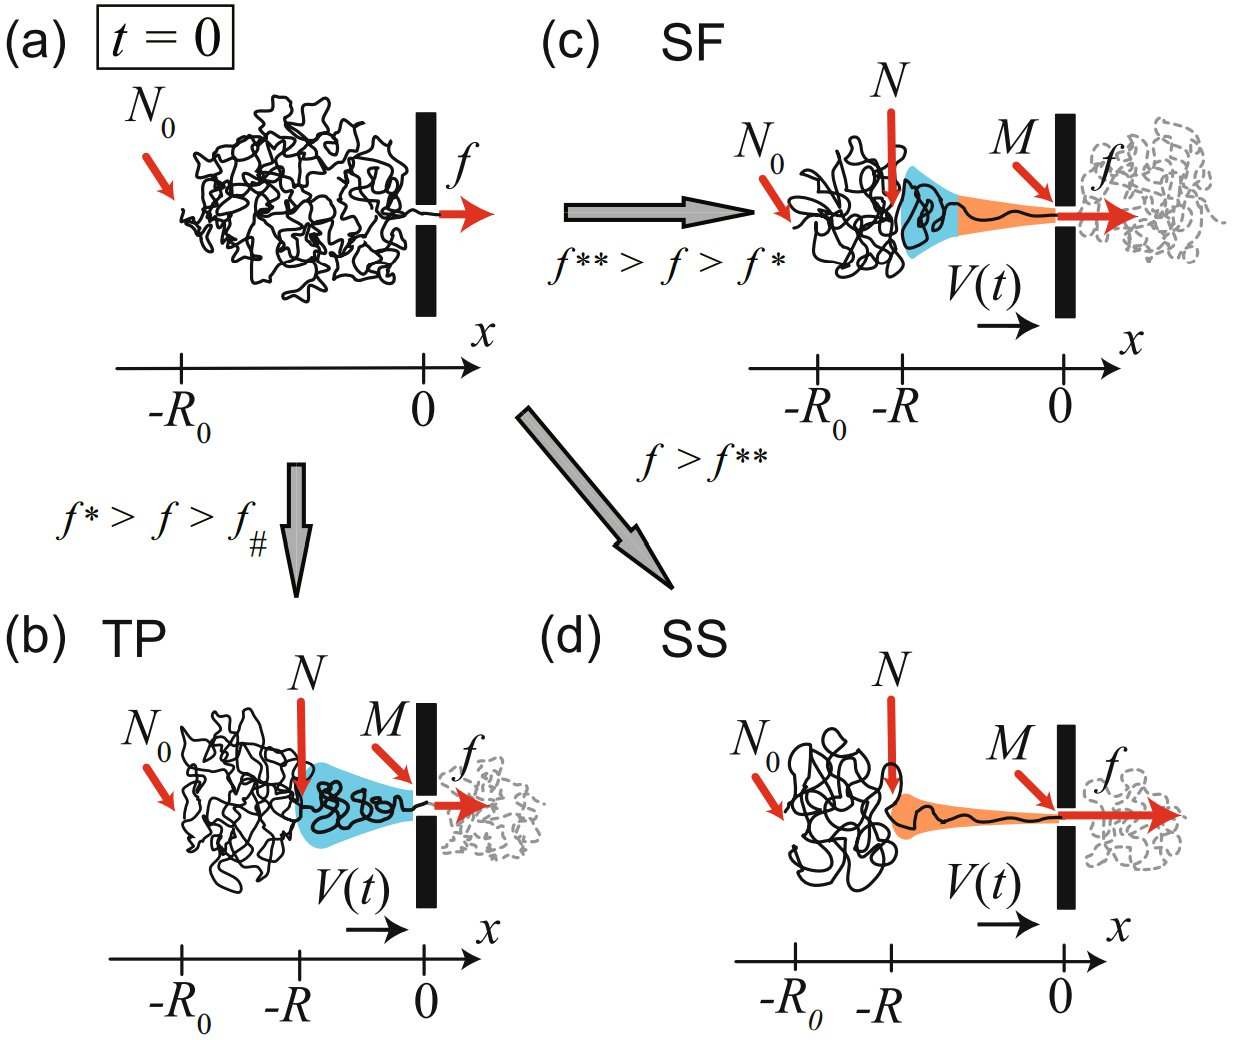
\includegraphics[width=0.8\textwidth]{regimesprofiles.jpg}
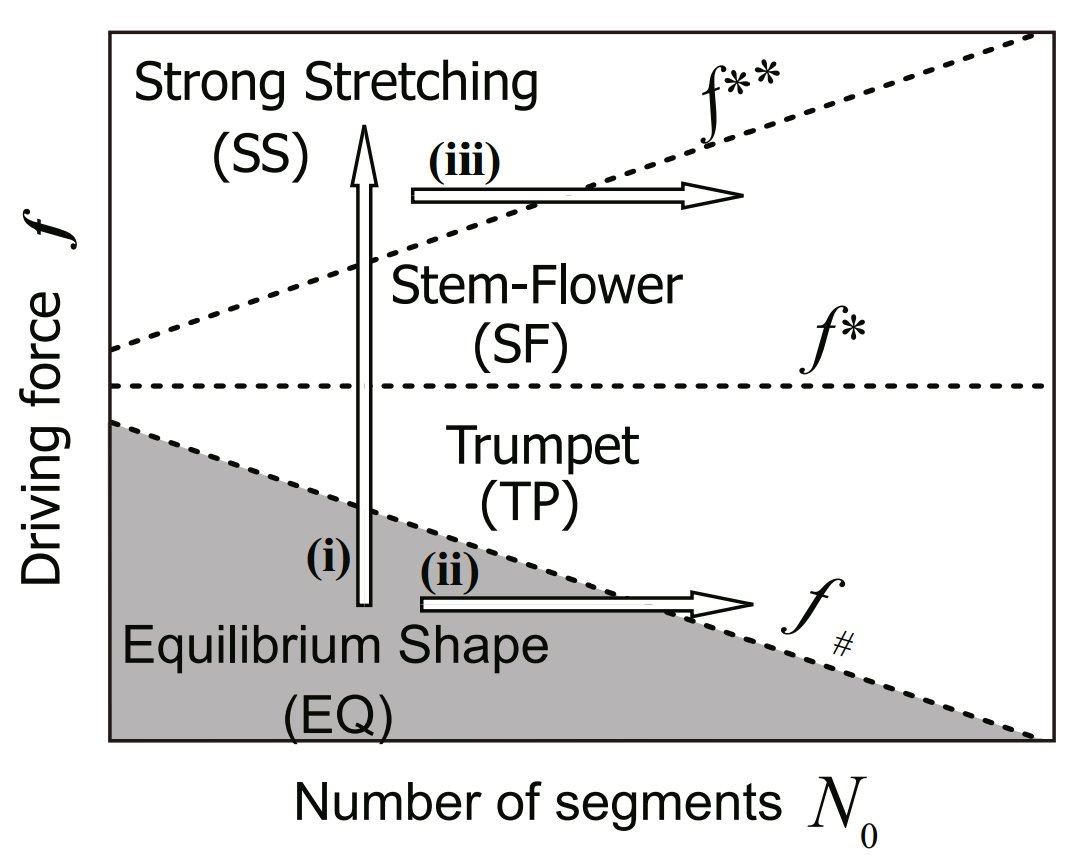
\includegraphics[width=0.5\textwidth]{regimedistrib.jpg} 

\caption[Régimes possibles au cours de la translocation]{Régimes proposés par Sakaue \cite{Saito2011}. (a) Régime d'équilibre (EQ) lors des translocation très lentes. (b) Régime trompette (TP): propagation de la tension le long de blob jusqu’au front où le polymère est à l'équilibre . (c) Régime Tige-fleur (SF: Stem-Flower): Une partie du polymère sous tension est étirée. (d) Régime d'étirement fort (SS: Super-Stretched): La totalité du polymère qui ressent la tension est étirée. La frontière entre les régimes (EQ) et (TP) $f_{\#}$ décroit en $N^{-\nu}$. La valeur $f^*$ entre les régimes (TP) et (SF) correspond à $f_c$ que nous avons défini au \hyperref[fc]{chapitre précédent}. La frontière entre (SF) et (SS), $f^{**}$, évolue elle en $N^{\nu}$. }
\label{regimeprofiles}
\end{center}
\end{figure}
 
  Pour une force très faible (régime avec $\alpha$ compris entre $2+\nu$ et $1+2\nu$), le polymère est toujours à l'équilibre et la translocation est lente, Il n'y a pas propagation de la tension le long de la chaîne car les fluctuations thermiques dominent. Pour une force qui augmente, mais qui ne dépasse pas la valeur $f_c$ définie au \hyperref[fc]{chapitre 2} on observe un régime en trompette. Le polymère présente alors des blobs de tensions jusqu'au front de propagation de la tension qui sépare les blobs de la partie toujours à l'équilibre. Ensuite apparaît le régime tige fleur. Pour une force supérieure à $f_c$, une partie du polymère est en extension comme dans le \hyperref[fc]{chapitre 2}, jusqu'à ce que la tension retombe à $f_c$ (partie tige), puis on observe un schéma similaire au régime trompette (partie fleure composée des blobs et de la partie à l'équilibre). A force très importante, s’installe le régime d'étirement fort. Le polymère est composé d'une partie étirée jusqu'au front de propagation et d'une partie à l'équilibre qui n'a pas encore ressenti la force. Sakaue et al.\cite{Saito2011} trouvent alors dans les 3 régimes (TP), (SF) et (SS), $\alpha=1+\nu$ et des valeurs de $\delta$ définies pour chaque régime. Ce modèle est alors utilisé et corrigé par plusieurs travaux \cite{Ambjrnsson2005,2Ambjrnsson2005,Rowghanian2011,Dubbeldam2012}. 
  
  
La continuation la plus pertinente de ces travaux provient de Ikonen et al., qui ont construit la théorie de la propagation de la tension-dynamique brownienne  (Brownian Dynamics-Tension Propagation theory ou BDTP) \cite{Ikonen2012,2Ikonen2012,Ikonen2013}. Leur théorie est basée sur la combinaison de la dynamique brownienne appliquée à la coordonnée de réaction (le nombre de monomères ayant effectué la translocation) avec une description explicite de la propagation du front de tension dans la chaîne qui génère un terme de mémoire dépendant du temps. Cette théorie prédis que $\alpha=1+\nu$ dans les trois régimes (TP, SF et SS) lorsque N tend vers l'infini. En ce qui concerne l'exposant lié à la force, un passage de $\delta \approx 0.9$ à $\delta=1$ pour les fortes forces est prédit \cite{Ikonen2013}.

\begin{figure}[H]
\begin{center}
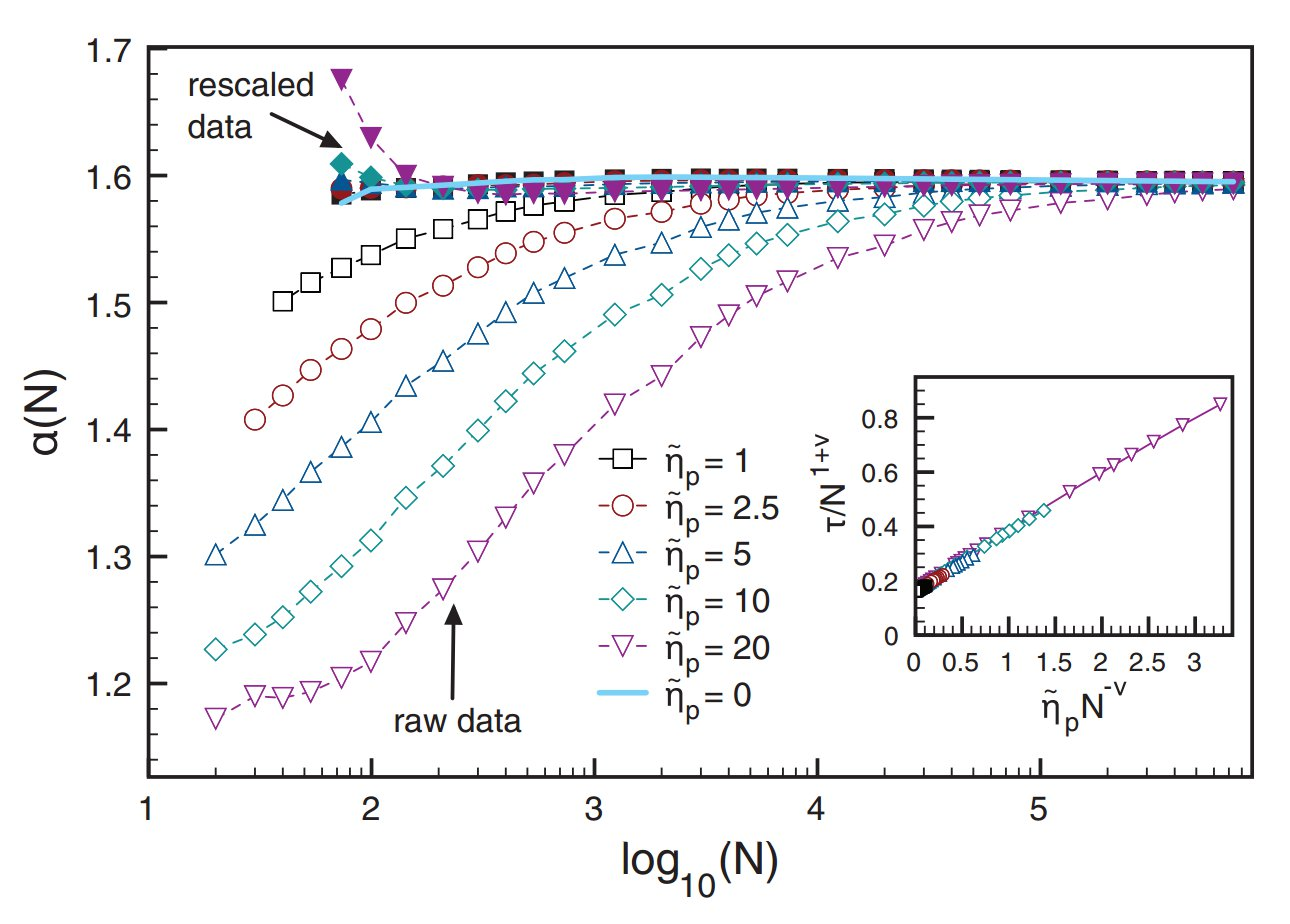
\includegraphics[width=0.9\textwidth]{bdtpalpha.jpg}

\caption[Evolution de $\alpha$ selon la théorie BDTP]{Evolution du paramètre $\alpha$ en fonction de la friction prévue par la théorie BDTP \cite{Ikonen2013}. Lorsque N tend vers l'infini, la limite est $\alpha=1+\nu$. Les simulations numériques usuelles trouvant des valeurs inférieures n'utilisent pas des valeurs de N suffisamment élevées.}
\label{bdtp}
\end{center}
\end{figure}

L'aspect le plus intéressant de cette théorie est qu'elle permet d'expliquer la large disparité des valeurs de $\alpha$ trouvées dans la littérature. En effet, le terme correctif lié à la propagation de la tension est assez grand et linéaire en N, ce qui explique que même pour des valeurs aussi élevée que $10^5$, $\alpha$ soit sous évalué (voir figure \ref{bdtp}). Ce terme correctif est physiquement en partie du à la phase dite de rétractation de la queue du polymère (voir figure \ref{tailretractation}). Dans leur article de revue, Palyulin, Ala-Nissila et Metzler \cite{Palyulin2014} présentent un tableau de comparaison entre cette théorie et des simulations numériques de plusieurs références. 



\begin{figure}[H]
\begin{center}
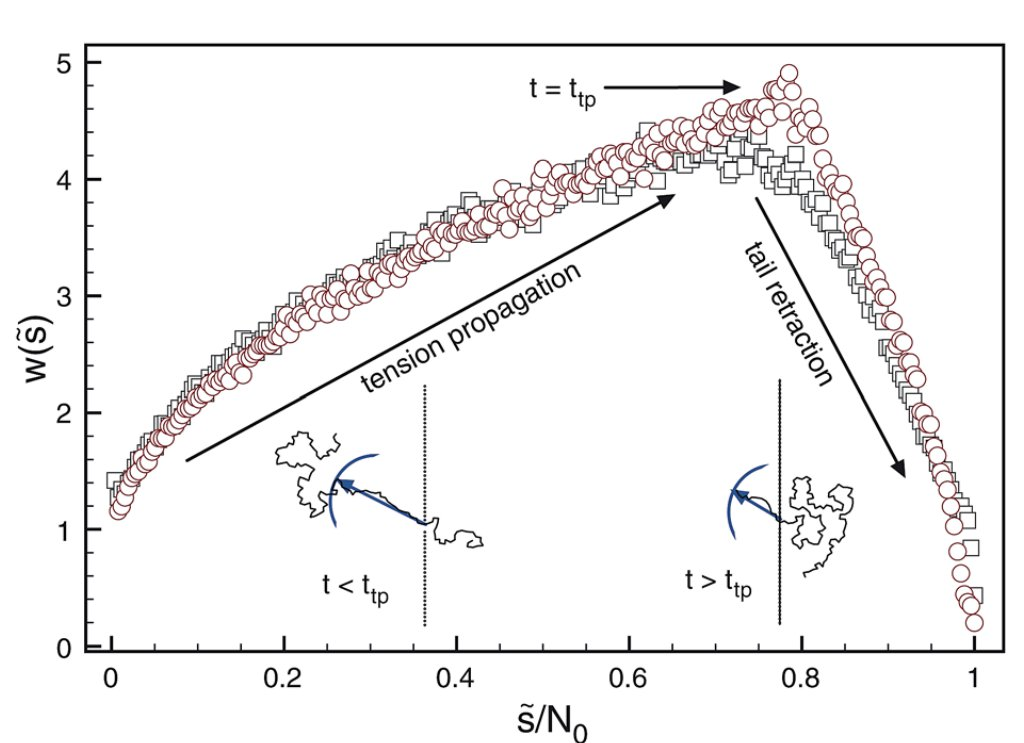
\includegraphics[width=0.75\textwidth]{tailretractinpore.jpg}
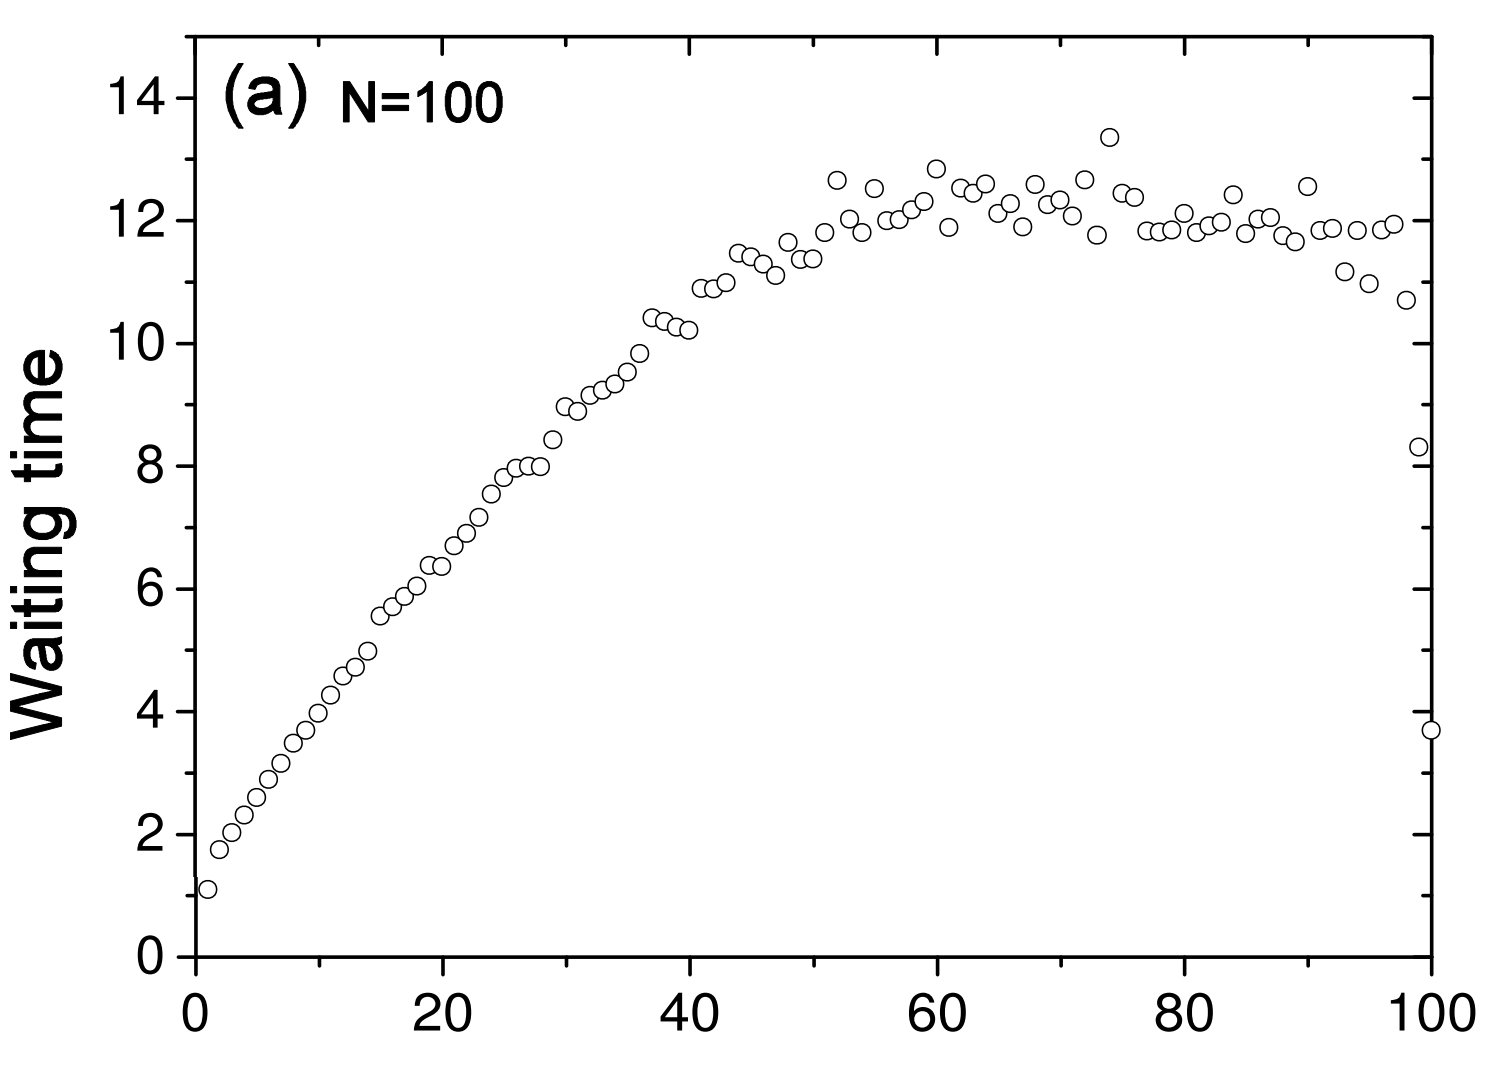
\includegraphics[width=0.75\textwidth]{tailretractpulling.jpg} 

\caption[Temps d'attente et rétractation de la queue du polymère]{Temps d'attente des monomères et rétractation de la queue du polymère en fin de translocation. Le temps d'attente d'un monomère est le temps moyen qu'il passe au sein du pore. Haut: cas d'une force exercée au sein du pore \cite{2Ikonen2012}. La rupture de la pente correspond à la période de rétractation de la queue du polymère, la tension s'est entièrement propagée au bout du polymère dont la translocation s'accélère. Bas: cas d'un polymère tiré \cite{Huopaniemi2007}. La rupture de pente se fait sur un plateau.}
\label{tailretractation}
\end{center}
\end{figure}

Cependant, leur prévision $\delta=1$ pour les fortes forces semble ne pas être vérifiée dans les simulations de dynamiques moléculaires \cite{2Ikonen2012}. Certains auteurs avancent une explication liée à l'encombrement du pore du côté trans \cite{Palyulin2014}, d'autres privilégient une influence d'une friction trop forte et/ou de liens trop faibles dans les simulations de dynamique moléculaire \cite{2Ikonen2012}. Pour la translocation forcée par une force située au sein du pore, la théorie BDTP est aujourd'hui celle qui semble la plus robuste.\\


En ce qui concerne le cas du polymère tiré par une de ses extrémités, les travaux sont beaucoup moins nombreux \cite{Kantor2004,Grosberg2006,Huopaniemi2007,Panja2008}. Pourtant, l'évolution du temps d'attente moyen des monomères présenté dans la figure \ref{tailretractation} ou la distribution du polymère au cours de la translocation présentée dans la figure \ref{translocshape}, montrent que les deux façons de forcer la translocation ne sont pas équivalentes.


\begin{figure}[H]
\begin{center}
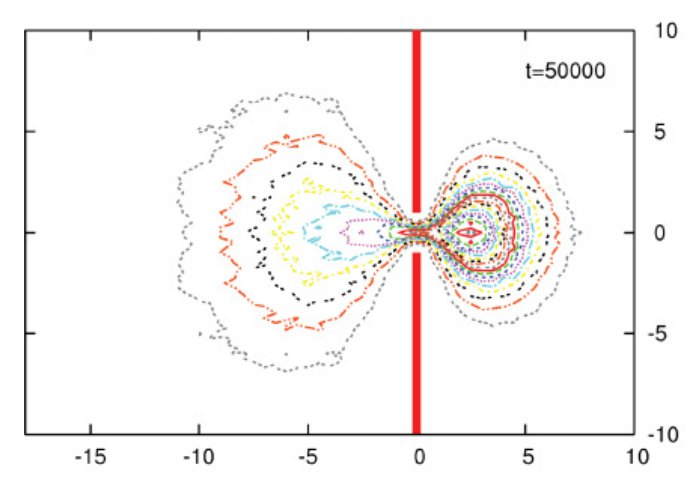
\includegraphics[width=0.49\textwidth]{transshapeintopore.jpg}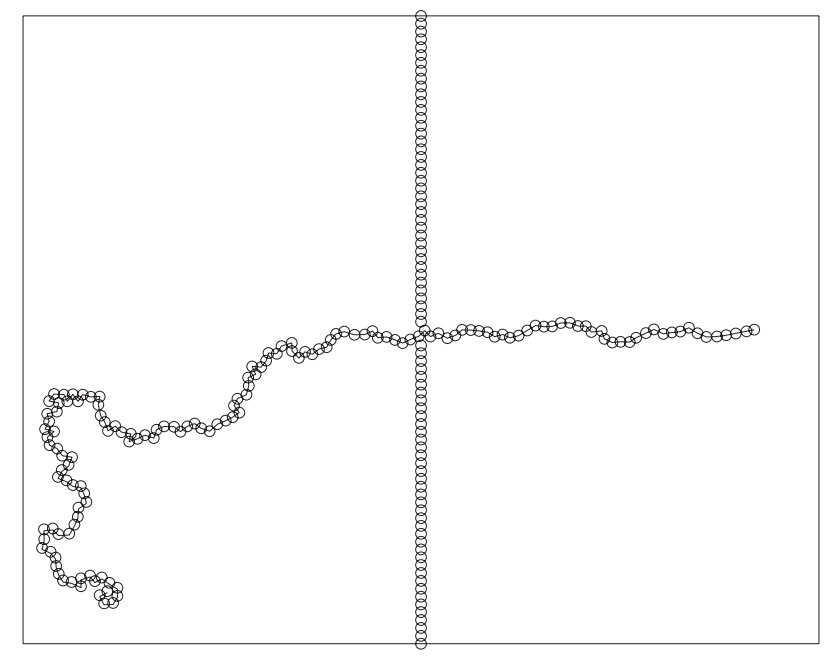
\includegraphics[width=0.49\textwidth]{shapetractiontransloc.jpg} 

\caption[Force dans le pore et force en bout de chaîne]{Différence entre force dans le pore et force en bout de chaîne. A gauche: Contours de distribution de type champignon du côté trans qui peut être encombré lorsque la force est générée au sein du pore \cite{Dubbeldam2012}. A droite: Configuration typique lorsque la force est exercée à une extrémitésdu polymère, la partie du polymère du côté trans est étirée et ne crée pas d'encombrement \cite{Huopaniemi2007}.}
\label{translocshape}
\end{center}
\end{figure}




Kantor et Kardar les premiers étudièrent ce cas \cite{Kantor2004} et prédirent $\tau \propto N^2/f^{2-\frac{1}{\nu}}$ pour un polymère idéal tracté à force faible (ce qui correspond à $f<f_c$, définie précédemment). Ces valeurs $\alpha=2$ et $\delta=2-\frac{1}{\nu}$ sont des valeurs limites obtenues par analyse d'échelle. Dans le cas d'une absence de membrane, le temps de translocation du polymère correspond à la distance à parcourir sur la vitesse moyenne. La vitesse moyenne est $V \propto f/N$. Pour la distance à parcourir, ils considèrent que le polymère est formé par loi d'échelle d'une succession de blobs comprenant $N_{B} \propto (k_BT/bf)^{-\nu}$ monomères de taille $ R_{B} \propto bN_B^{\nu}\propto k_BT/f$, il y a un nombre de blobs successifs $N/N_B \propto N (fb/k_BT)^{1/\nu}$. La distance à parcourir est  $L \propto R_B(N/N_B) \propto bN(fb/k_BT)^{\frac{1}{\nu}-1} $. On peut alors déduire $\tau \propto \frac{L}{V} \propto N^2/f^{2-\frac{1}{\nu}}$. Nous remettons en cause cette vision avec les travaux de Sakaue \cite{Sakaue2012} vus au \hyperref[fc]{chapitre précédent} qui rebutent l'image de blobs successifs de taille similaire au profit de blobs de taille croissante ; l'élongation $L$ est alors proportionnelle à $Nf$. On a donc plutôt $\tau \propto \frac{L}{V} \propto N^2/f^{2}$. Cette remarque ne modifie pas la valeur limite de $\alpha$ prévue,  de plus la forme trompette ainsi envisagée est incompatible avec le passage au sein du pore qui va limiter la taille des blobs .

 Kantor et Kardar avancent alors que la même valeur de $\alpha$ est attendue dans le cas du modèle de Rouse. Cette affirmation se base sur l'argument suivant: la chaîne est étirée du coté trans (elle ne subie alors aucune influence de volume exclu) et c'est entièrement ce côté qui va piloter la translocation. Ils vérifient alors leurs prédictions par simulation de type Monte-Carlo à 2 dimensions. Pour le polymère idéal, ils trouvent $\alpha =1.936 \pm 0.01$, valeur en augmentation avec la longueur de la chaîne (les effets de tailles finis réduisent la valeur de $\alpha$) et confirment une loi asymptotique de $\alpha=2$. Dans le cas d'un polymère de Rouse, ils trouvent $\alpha =  1.875 \pm 0.005$, également en augmentation et avancent donc un comportement asymptotique de $\alpha=2$. En ce qui concerne la valeur de $\delta$, la figure \ref{deltakantor} montre un comportement asymptotique qui se rapproche de $1/f$. 
% Notre remarque porte sur la valeur de $\delta$, or on s'attend à une transition de $\delta=0$ pour les forces faibles (cas proche de la translocation non biaisée) à une limite asymptotique qui ne peux pas être supérieure à $\delta=1$. La  valeur de 2 que nous proposons ne se situe pas dans cet intervalle [0:1], contrairement à la valeur $\delta=2-\frac{1}{\nu}$.
 %et l'origine ayant un comportement linéaire conforte notre estimation d'exposant $\delta$.
 
 \begin{figure}[H]
\begin{center}
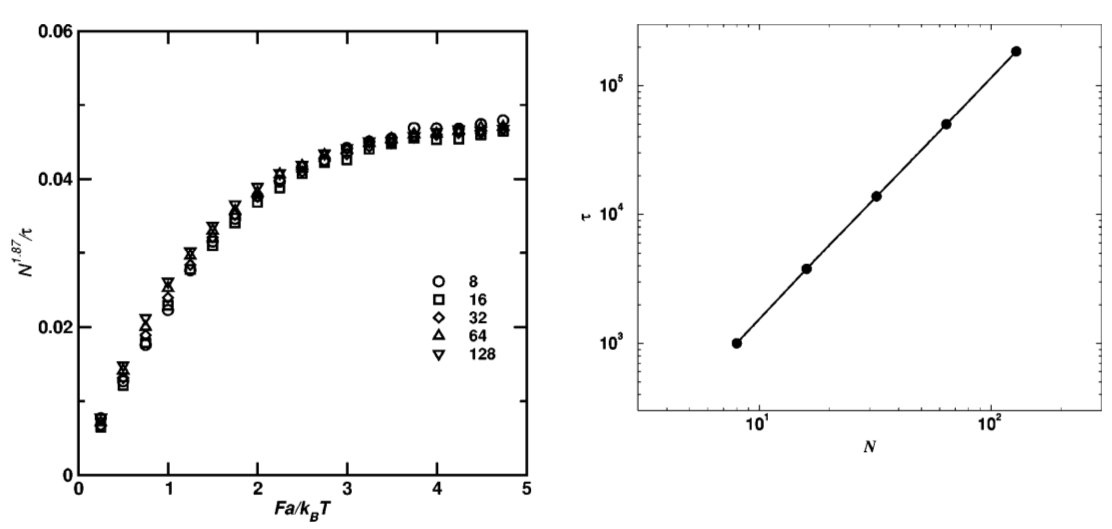
\includegraphics[width=1\textwidth]{kantorkardar.jpg}
\caption[Exposants critiques pour une translocation tractée]{ A forte force, Kantor et Kardar \cite{Kantor2004} trouvent  $\alpha=1.875$ et $\delta=1$. A droite: estimation de $\alpha$. A gauche: graphe réajusté dont le plateau à haute force montre que $\delta=1$.}
\label{deltakantor}
\end{center}
\end{figure}

Ces valeurs sont confirmées par Huopaniemi et al. \cite{Huopaniemi2007}, ainsi que par Panja et Barkema pour la valeur à forte force \cite{Panja2008}. Ces derniers contestent cependant la valeur à faible force qui revient au cas de la translocation non biaisée (notons que ce papier est antérieur à d'autres travaux qu'ils ont réalisé dont nous avons parlé précédemment et qui reportaient une transition entre exposants $1+2\nu$ et $2+\nu$ dans le cas de la translocation non biaisée \cite{Panja22010}).

 Dans leurs travaux, Huopaniemi et al. \cite{Huopaniemi2007} analysent également le cas de la translocation à travers un pore infiniment large. Malgré le fait que l'article correspondant ne détaille pas comment ce pore infiniment large est implémenté ( S'agit-il d'une translocation sans membrane ? Les configurations initiales sont générées contre une membrane puis celle ci disparaît lors de la phase de translocation ? Utilisent-ils un pore très grand devant le rayon de giration du polymère ? Quid de l'hypothèse d'un seul monomère au sein du pore à tout instant ? ), il est intéressant de remarquer qu'ils trouvent un régime unique pour leur pore standard et trois régimes différents pour le pore infiniment large (voir figure \ref{regimestransloctractee}).

\begin{figure}[H]
\begin{center}
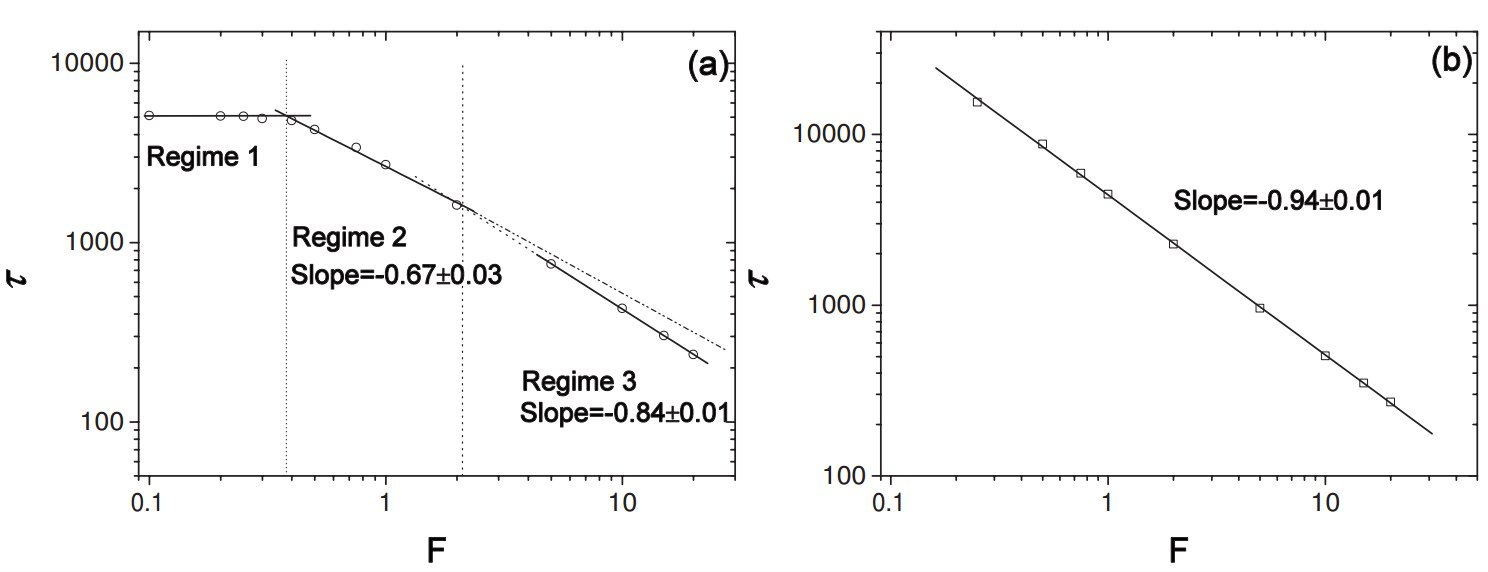
\includegraphics[width=1\textwidth]{regimespulling.jpg}
\caption[Régimes de forces pour une translocation tractée]{Translocation forcée en tirant le polymère par une de ses extrémités \cite{Huopaniemi2007}. (a) : translocation à travers un pore infiniment large, trois régimes sont observables. A faible force, la force n'influence pas le temps de translocation, on est alors proches du cas non biaisé. A force intermédiaire, $\delta$ augmente pour correspondre à 2/3, valeur anticipée par la loi d'échelle conduisant à $\delta=2-\frac{1}{\nu}$ pour ces simulations à deux dimensions. A forte force $\delta$ augmente encore pour se rapprocher de 1. (b) : Translocation à travers un pore non infiniment large. Un seul régime demeure avec $\delta$ proche de 1.}
\label{regimestransloctractee}
\end{center}
\end{figure}

Tâchons de comparer les trois régimes observés dans le cas du polymère tiré par une extrémité aux quatre du cas de la translocation biaisée par une différence de potentiel. A notre connaissance, aucun travaux ne porte sur le cas du polymère tracté en prenant en compte le modèle de Sakaue et al. ou la théorie BDTP. Le premier régime correspond dans les deux cas à une force faible et a un phénomène proche de la translocation non biaisée. Les régimes (TP) et (SF) présentés dans le cas de la translocation forcée par différence de potentiel ne sont plus pertinents dans le cas du polymère tiré. En effet la forme de la trompette est incompatible avec le passage à travers le pore. Lorsque le diamètre du col de la trompette est comparable à celui du pore, le mouvement est ralenti et le polymère s'étire du côté trans. On se retrouve alors avec la forme d'un des trois régimes (TP), (SF) ou (SS) du côté trans. avec pour taille de blob maximale des régimes (TP) et (SF), le diamètre du pore. A très forte force, on a l'équivalent du régime (SS) avec un front de propagation de la tension situé soit au niveau du pore, soit qui remonte du côté cis. 


%A force très importante, le polymère est entièrement étiré, on a le régime (SS) du côté cis dans le cas de la différence de potentiel.Pour le polymère tiré, le régime (SS) se situe des deux côtés de la membrane (le polymère est entièrement étiré de part et d'autre de la membrane jusqu'au front de propagation de la tension).

 Ces exposants sont également corroborés à forte forces dans un cas presque similaire, celui de la désorption de polymères \cite{Paturej2012}. En effet le cas d'un polymère attaché à une surface dont on tire une extrémité peut être vu comme le même problème avec une composante d'affinité avec le support d'absorption qui fait office de barrière énergétique à franchir. L'analogie est proche du cas d'un pore étroit ou il faudrait une force seuil pour amorcer la translocation. En ce qui concerne les exposants du cas de la translocation biaisée par une différence de potentiel, une analogie peut être faite avec l'ouverture et de la fermeture d'épingles dans l'ADN ou l'ARN \cite{Ferrantini2011}.


 \newpage

\subsection{Distribution du temps de translocation}

Dans leurs travaux sur la translocation, Daniel Y Ling et Xinsheng Sean Ling \cite{Ling2013} proposent d'étudier la distribution des temps de translocation en considérant la translocation comme un phénomène de diffusion biaisée unidimensionnelle. Ils considèrent le pore suffisamment fin comparé à la longueur du polymère pour être considéré comme un marcheur qui se déplace le long de ce dernier. Ils peuvent donc lui appliquer l'équation de Fokker-Planck:

\begin{eqnarray}
\frac{\partial P(x,t)}{\partial t} =   D\frac{\partial ^2 P(x,t)}{\partial ^2 x} - \nu \frac{\partial  P(x,t)}{\partial  x}
\label{equfokkerplank}
\end{eqnarray}

Avec $P(x,t)$ la probabilité pour le pore d'être à la coordonnée $x$ le long du polymère à l'instant $t$, $D$ le coefficient de diffusion et $\nu$ la vitesse du marcheur. Ils utilisent pour conditions aux limites, le premier monomère au sein du pore à $t=0$ et une absorption lorsque le pore atteint $L$ l'extrémité du polymère, il n'y a pas de retour possible:

\begin{eqnarray}
 P(x,0) =   \delta(x)\text{  }, \text{  } P(L,t)=0
\label{condlim}
\end{eqnarray}

La solution de l'équation différentielle est:

\begin{eqnarray}
 P(x,t) = \frac{1}{\sqrt{4\pi D t}} \left(e^{-\left(x-\nu t\right)^{2}/4Dt} -e^{(\nu L/D)}e^{-\left(x-2L-\nu t\right)^{2}/4Dt} \right)
\label{equfokkerplanksol}
\end{eqnarray}

La distribution du temps de translocation est la distribution du temps de premier passage:

\begin{eqnarray}
 F1(t) = -\frac{d}{dt}\int_{-\infty}^L  P(x,t) dx
\label{firstpassageint}
\end{eqnarray}

\begin{eqnarray}
 F1(t) = \frac{L}{\sqrt{4\pi D t^3}} e^{-\left(L-\nu t\right)^{2}/4Dt}
\label{firstpassage}
\end{eqnarray}

Avec l'équation \ref{firstpassage} ils arrivent à reproduire des résultats expérimentaux dans certaines conditions où la vitesse du marcheur peut être aisément reliée aux conditions expérimentales, les hypothèses $D$ et $\nu$ constants valables. Nous nous servirons de cette équation pour analyser les distributions de nos temps de translocation.





\section{Résultats numériques et théoriques}

Nous avons étudié trois cas différents dans le cadre de notre travail sur une membrane fixe. Dans un premier temps, la translocation d'un polymère non structuré à travers un pore suffisamment large pour limiter les frottements est expérimentée. Nous avons retiré 24 grains du centre de la membrane pour former le nanopore. Puis nous avons testé notre polymère structuré, également dans un pore suffisamment large, il a alors fallut retirer 54 grains. Pour terminer nous avons investigué l'effet d'un nanopore étroit sur la translocation du polymère structuré en retournant à un pore constitué par le retrait de 24 grains. Les deux pores utilisés sont présentés sur la figure \ref{bothpores}.
 \begin{figure}[H]
\begin{center}
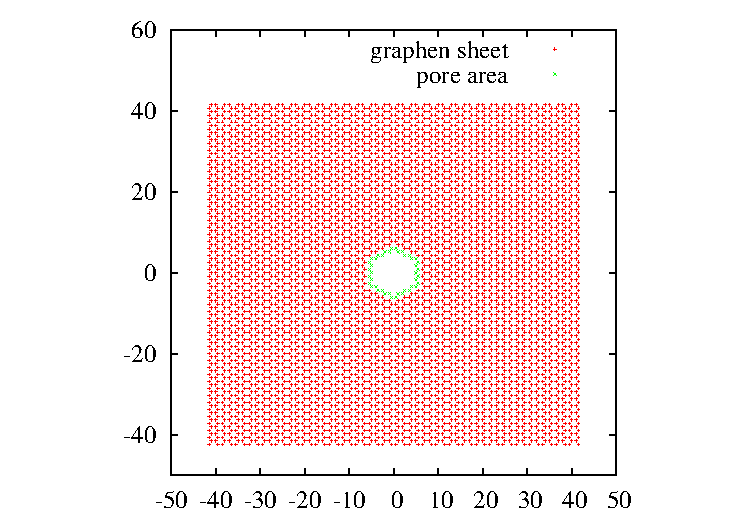
\includegraphics[width=0.45\textwidth]{holebigger.pdf} 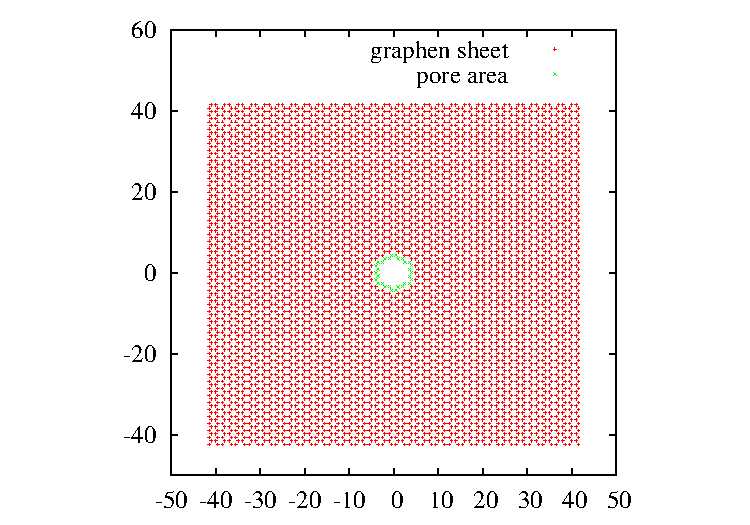
\includegraphics[width=0.45\textwidth]{holesmall.pdf}

\caption[Nanopores utilisés]{Les deux nanopores utilisés. A gauche: Pore large pour la translocation de polymères structurés. A droite: Pore étroit pour la translocation de polymères structurés et larges pour des polymères simples linéaires. Un zoom sur les pores et la taille relative des grains du polymère en cours de translocation seront fournis par la suite  pour chaque expérience.}
\label{bothpores}
\end{center}
\end{figure}

\subsection{Translocation du polymère simple}


Afin d'avoir une base de comparaison, nous avons étudié le cas du polymère linaire simple dont nous avons étudié la translocation à travers un nanopore relativement large (voir figure \ref{porelargesimplepol}). Cette base nous servira aussi bien de vérification par rapport à la littérature existante que d'étalon pour notre polymère structuré.


\begin{figure}[H]
\begin{center}
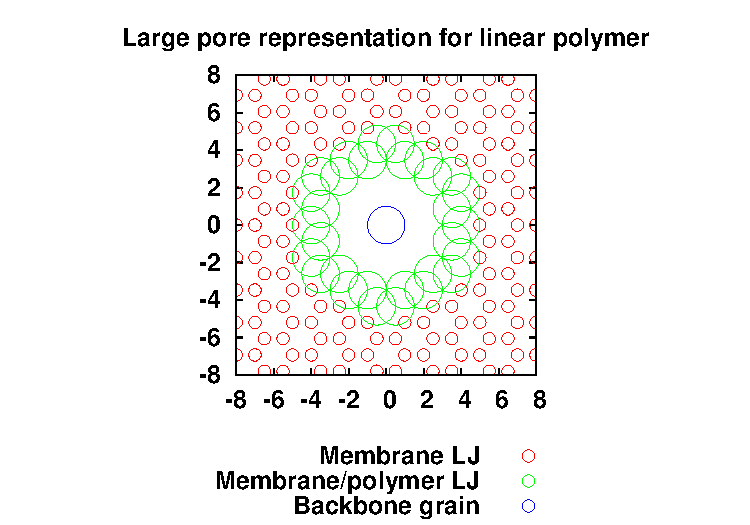
\includegraphics[width=1\textwidth]{simplepolpore.pdf}


\caption[Polymère simple dans le pore]{Pore large utilisé pour la translocation de notre polymère linéaire simple. Les tailles des différents grains sont respectées. }
\label{porelargesimplepol}
\end{center}
\end{figure}

Les grains de la membrane interagissent avec le polymère avec des potentiels de Lennard-Jones tel que $\sigma_{mp}=1$ soit supérieur au pas du réseau. Nous sommes alors sûrs que le polymère ne peut pas pénétrer la membrane ailleurs qu'au sein du pore.\\

\begin{figure}[H]
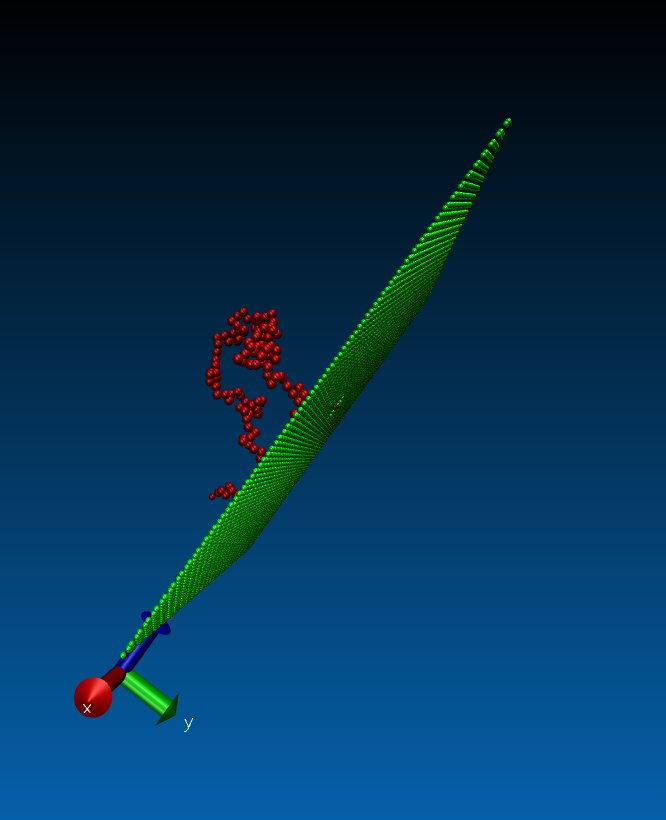
\includegraphics[width=0.5\textwidth]{simplepoltransloc1.jpg}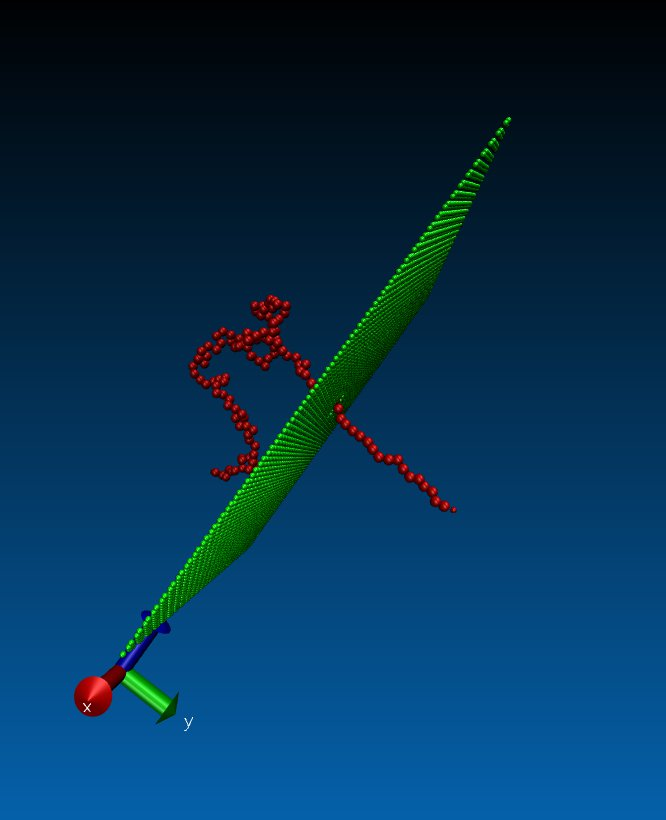
\includegraphics[width=0.5\textwidth]{simplepoltransloc2.jpg}
\begin{minipage}{0.5\linewidth}
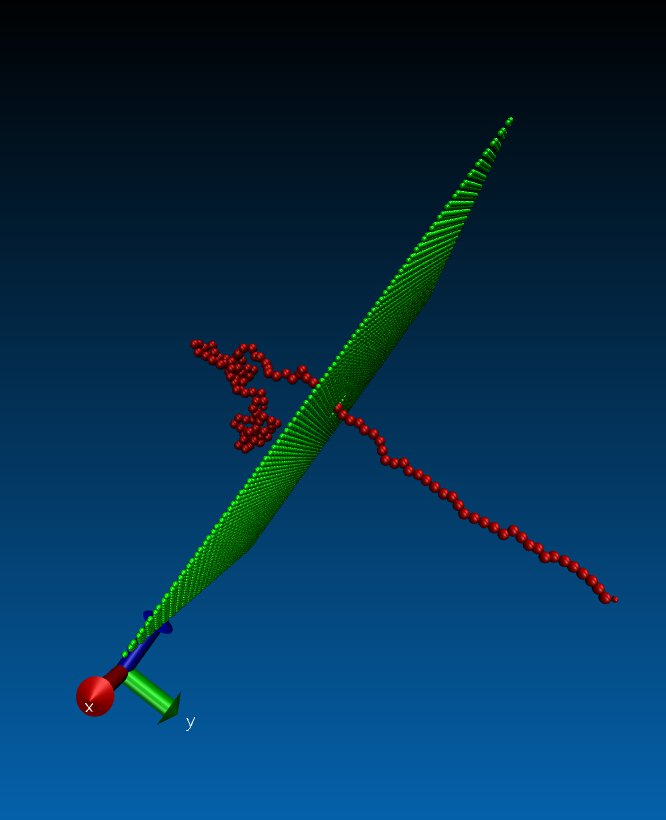
\includegraphics[width=\textwidth]{simplepoltransloc3.jpg}
\end{minipage}
\begin{minipage}{0.5\linewidth} 
\caption[Capture d'écran de la translocation du polymère simple]{Captures d'écran au cours d'une translocation typique.La partie du côté cis conserve une conformation en pelote, le côté trans est en extension. Cela laisse entrevoir un côté cis à l'équilibre dominé par les fluctuations thermiques et un côté trans dominé par la force exercée à l’extrémité du polymère. Nous reviendrons sur cet aspect lors de l'élaboration d'un cadre théorique pour traiter la translocation d'un polymère tracté.}
\label{screenshotspolsimple}
\end{minipage}
\end{figure}



\noindent Après avoir généré les 1000 configurations d'équilibre, nous tentons d'effectuer 1000 translocations sur une plage de valeurs de force comprises entre 0.1 et 100 unité de Lennard Jones. Nous avons étudié 3 polymères de taille 16, 32 et 64 grains, un quatrième de 128 grains est partiellement étudié afin d'estimer des valeurs de $\alpha$ sur plus de trois points. Une translocation typique est montrée sur la figure \ref{screenshotspolsimple} et la figure \ref{taupolsimple} présente les résultats que nous avons obtenus.
 
\begin{figure}[H]
\begin{center}
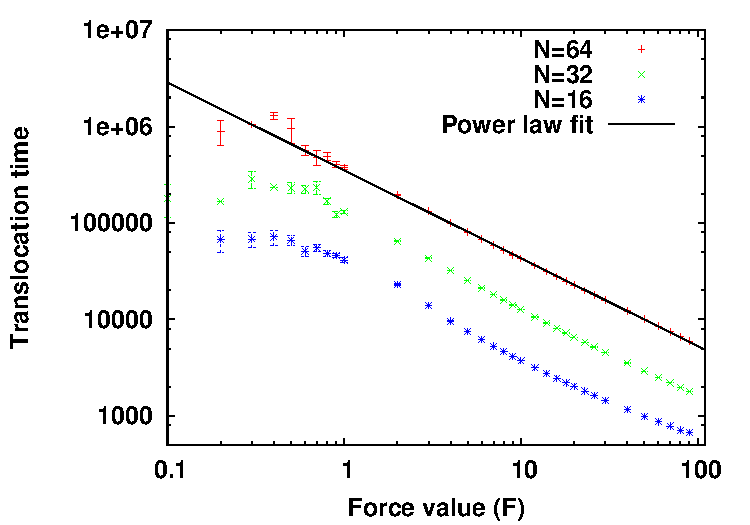
\includegraphics[width=0.9\textwidth]{translocpolsimple.pdf} 
\caption[Temps de translocations du polymère simple]{Temps de translocation moyen du polymère en fonction de la force de traction exercée. A faible forces, un plateau semble indiquer  que nous nous situons dans le régime proche de la translocation non biaisée. Lorsque la force est plus importante, la valeur moyenne du temps de translocation décroit d'une manière qui semble proportionnelle à l'inverse de la force exercée.}
\label{taupolsimple}
\end{center}
\end{figure}

On peut clairement distinguer un plateau à faibles forces et une rupture de pente suivie de la décroissance du temps de translocation lorsque la force augmente. A l'aide de ses données brutes, tâchons d'estimer les valeurs de $\alpha$ et $\delta$. Pour $f<1$ nous sommes sur le plateau et nous estimons $\alpha=2.01 \pm 0.05$ pour $f=0.5$. Pour $f>1$, notre estimation est $\alpha=1.84 \pm 0.01$ pour $f=30$. La figure \ref{ndeppolsimple} présente les valeurs de $\alpha$ trouvées dans ces deux régimes. Ces résultats sont inférieurs aux valeurs théoriques prévues car nous avons des polymères relativement courts.

\newpage


\begin{figure}[H]
\begin{center}
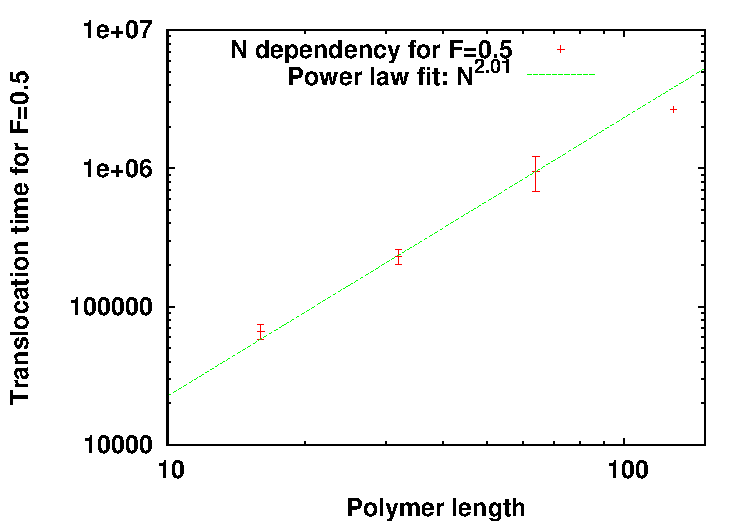
\includegraphics[width=0.9\textwidth]{ndeppolsimplef05.pdf}
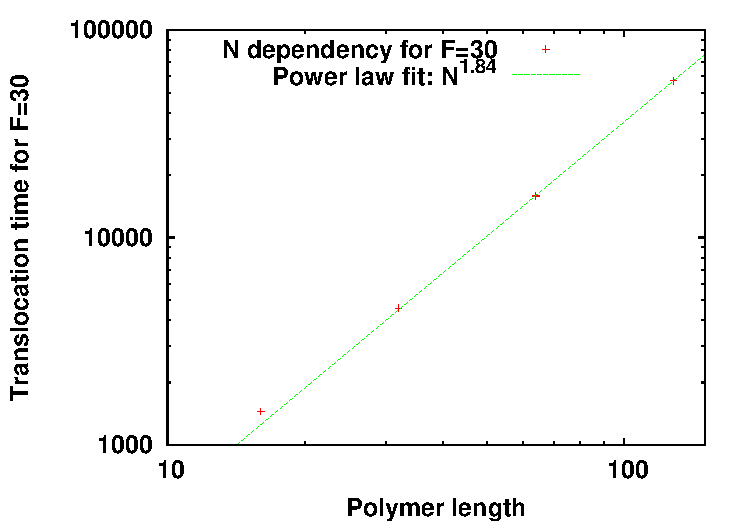
\includegraphics[width=0.9\textwidth]{ndeppolsimplef30.pdf}

\caption[Temps de translocations en fonction de N]{Evolution du temps de translocation moyen avec N. En haut, pour une faible force, nous estimons $\alpha=2.01 \pm 0.05 $ (la valeur pour N=128 étant réalisée sur une translocation unique, elle n'a pas été prise en compte dans le calcul de $\alpha$), pour une valeur théorique attendue $\alpha=1+2\nu \approx 2.18$ pour une translocation non biaisée. En bas, pour une force modérée, $\alpha= 1.84 \pm 0.01$, pour une valeur théorique attendue de 2. Nos valeurs de $\alpha$ sont sous estimées à cause d'effets de taille finie car nos polymères sont courts.}
\label{ndeppolsimple}
\end{center}
\end{figure}

\newpage


Afin de visualiser les différents régimes, nous avons retracé les temps de translocation de manière réajustée. Connaissant $\alpha$ dans le régime décroissant et soupçonnant une valeur de $\delta$ proche de 1, nous avons retracé $\tau \cdot f/N^{\alpha}$ (avec $\alpha=1.84$). Les résultats obtenus sont présentés sur la figure \ref{simplepolrescale}.


\begin{figure}[H]
\begin{center}
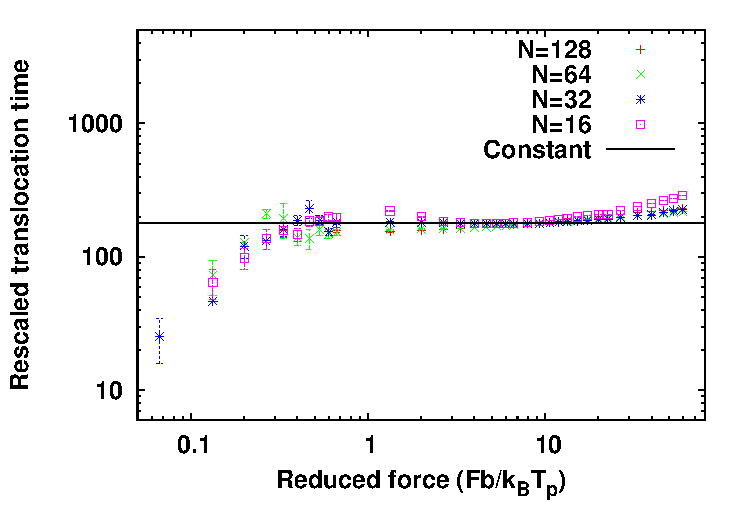
\includegraphics[width=0.9\textwidth]{transloctaufsimplepolresc.pdf}


\caption[Temps de translocations réajustés]{Temps de translocation réajusté en fonction de la force exercée. La force réduite correspond à la division de l'échelle d'énergie donnée par la force par celle donnée par la température. On observe clairement une rupture de pente qui traduit le changement de régime entre translocation non biaisée et translocation forcée. Lorsque la force est intermédiaire, $\delta=1$, comme attendu, cependant à forte force, on observe une diminution de $\delta$, avec $\tau \propto f^{-0.82}$.}
\label{simplepolrescale}
\end{center}
\end{figure}

Ce réajustement des temps de translocation permet d'observer, à forte force, une diminution de $\delta$ qui sature à 0.822 $\pm$ 0.006 . Nous avons vu que dans la littérature, ce comportement apparaît aussi bien dans le cas de la translocation forcée par différence de potentiel que dans le cas de la force de traction à une extrémité. Cette situation semble éliminer l'explication avancée concernant un effet d'encombrement dû au polymère du côté trans \cite{Palyulin2014}. Nous nous proposons de tester l'hypothèse de liaisons et/ou friction du solvant trop faible/forte \cite{2Ikonen2012}. 

Nous nous sommes placés dans un cas simple, déterministe, aisément soluble numériquement. Le polymère est placé perpendiculairement à la membrane avec le premier monomère au milieu du pore. La température est nulle, nous faisons varier $\nu$, le coefficient de frottement des grains avec le solvant et $k$, la constante de raideur associée aux liaisons entre grains. Les résultats que nous obtenons, présentés dans le tableau ci-dessous, permettent d'accréditer l'hypothèse de liaisons et/ou friction trop faible/forte.

\begin{table}[H]
\begin{center}
\setstretch{1.2}
\begin{tabular}{|c|c|c|}
  \hline
  Valeur de $\nu$ & Valeur de $k$ & Valeur de $\delta$ \\
  \hline
  0.1 & 30 & 0.989 $\pm$ 0.007\\
  0.33 & \_  & 0.972 $\pm$ 0.004 \\
  1 & \_ & 0.884 $\pm$ 0.05  \\
  3 & \_  &  0.62 $\pm$ 0.02  \\
  10 & \_  &  0.51 $\pm$ 0.02 \\
  30 & \_  &  0.478 $\pm$ 0.02  \\
  1 & 3  &  0.85 $\pm$ 0.02  \\
  1 & 300  &  0.90 $\pm$ 0.02\\
  \hline
 
    
\end{tabular}
\caption[Influence de la friction et de la force des liaisons sur le comportement à forte force]{Valeurs de $\delta$ trouvées à fortes forces pour différents paramètres de friction et de force de liaison en supprimant le bruit thermique. Simulations déterministes réalisées sur un polymère composé de 16 grains alignés à l'équilibre perpendiculairement à la membrane, le premier grain sur lequel s'applique la force situé au centre du pore. Ces valeurs permettent d'expliquer les valeurs de $\delta$ inférieure à 1 à fortes forces.}  

\end{center}

\end{table}

Cette hypothèse semble validée, dans le cas où il n'y a pas de température. Elle semble donc très probable dans le cas normal pour lequel nous trouvons un exposant 0.82 légèrement inférieur au 0.88 de cette étude.

\begin{figure}[H]
\begin{center}
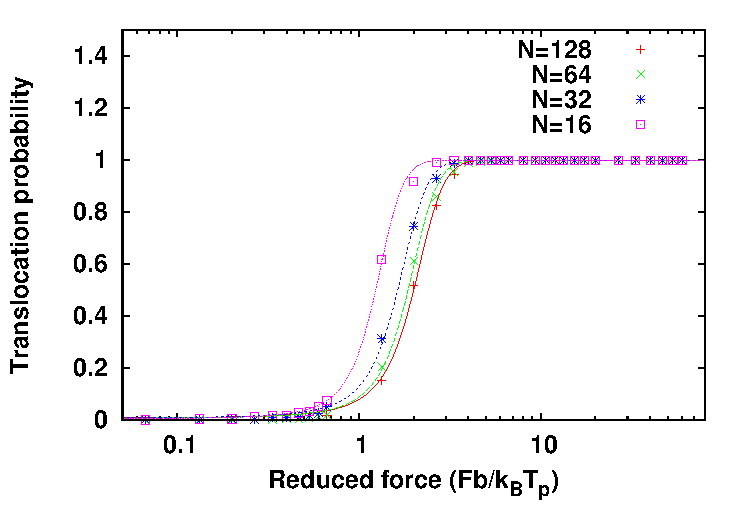
\includegraphics[width=0.9\textwidth]{probatranslocsimplepol.pdf}


\caption[Probabilité de translocation du polymère simple]{Probabilité de translocation du polymère linéaire simple côté trans. Plus le polymère est long, plus il va falloir une force importante pour effectuer la translocation avec succès.}
\label{probatranslocpolsimple}
\end{center}
\end{figure}

Regardons maintenant l'autre extrémité de la plage de forces appliquées. Dans le cas des forces très faibles, beaucoup de translocations sont avortées du fait de la sortie côté cis. On a une probabilité de translocation qui est liée à la force appliquée et à la taille du polymère, comme le montre la figure \ref{probatranslocpolsimple}.



Nous avons analysé nos données avec une fonction de type:

\begin{eqnarray}
P(f) =  \frac{1}{\left( 1+\exp\left(-\frac{f-f_{0}}{\Delta f} \right) \right)} 
\label{probtransloc}
\end{eqnarray}
 
$f_{0}$ étant la force nécessaire pour obtenir une probabilité de translocation de 1/2. Nous n'avons pas trouvé de loi particulière suivie par ces deux paramètres. Une étude de leur variations avec la température pourrait être utile mais s'avère très coûteuse numériquement.\\ 

Intéressons nous maintenant à la distribution de nos temps de translocation. En nous plaçant sur la plage donnant $\delta=1$, nous pouvons faire l'hypothèse que la vitesse moyenne de la translocation est proportionnelle à la force appliquée en bout de chaîne.  Nous avons fitté nos distributions de temps de translocation avec l'équation \ref{firstpassage} présentée dans la partie précédente. Des exemples de distributions sont présentés sur la figure \ref{distribpolsimple}.

\begin{figure}[H]
\begin{center}
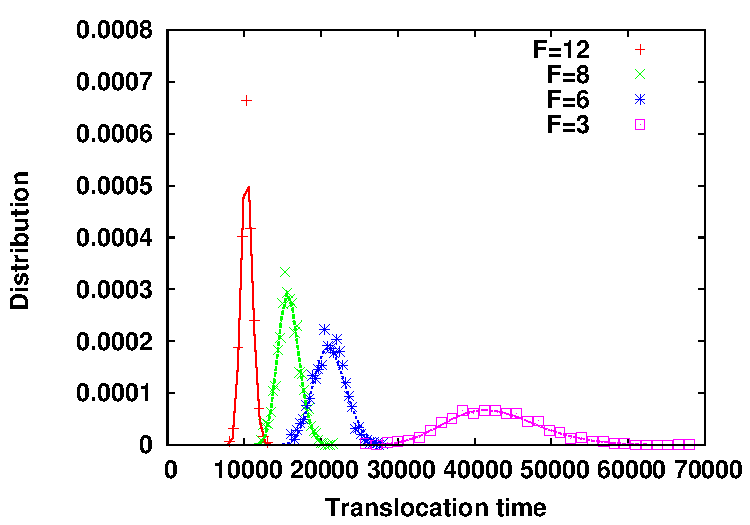
\includegraphics[width=0.9\textwidth]{distribpolsimple.pdf}


\caption[Distribution des temps de translocation du polymère simple]{Distribution des temps de translocation d'un polymère linéaire simple constitué de 32 grains. La formule proposée par D.Y. Ling et X.S Ling \cite{Ling2013} reproduit bien nos distributions et permet d'évaluer une vitesse moyenne de translocation.}
\label{distribpolsimple}
\end{center}
\end{figure}

Puisque la distribution proposée ne présente que deux paramètres, regardons comment les interpréter. Le premier paramètre correspond au coefficient de diffusion de la membrane le long du polymère, l'algorithme de fit que nous avons utilisé est très peu sensible sur cette valeur, de larges plages sont considérées comme satisfaisantes. Le deuxième paramètre, quand à lui est bien plus précis. Nos coefficient de diffusion restent relativement constants (comme attendu),  pour nos vitesse de biais du marcheur en revanche nous avons une évolution linéaire avec la force appliquée sur la zone où $\delta=1$, voir figure \ref{frictionpolsimple}. Le fit utilisé dans le cas $v \propto \mu E$ d'un gradient de potentiel électrique \cite{Ling2013} est un choix également pertinent ici dans notre cas: $v \propto f/\xi$.




\begin{figure}[H]
\begin{center}
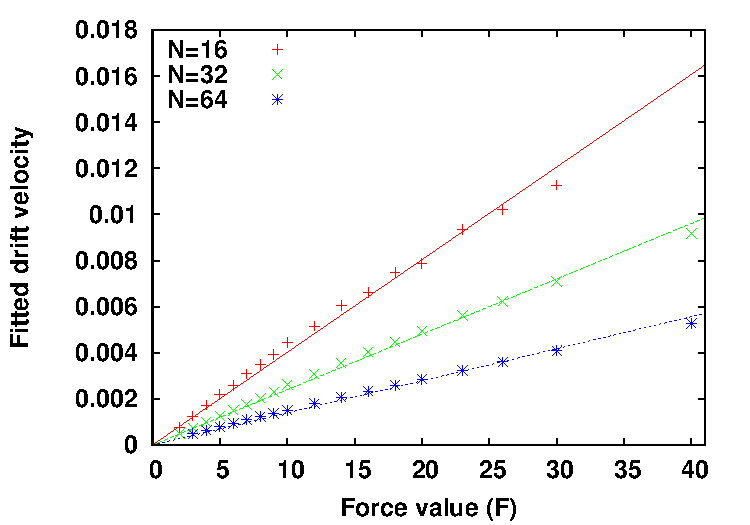
\includegraphics[width=0.9\textwidth]{retestfrictioncoeffsimplepolrescaled.pdf}


\caption[Friction et translocation, polymère simple]{Estimation de la vitesse de biais lors de la diffusion de la membrane le long du polymère constitué d'une chaîne simple de 16, 32 et 64 grains. Notre fit donne le paramètre $v/L$ dont nous extrayons $v$ en multipliant le paramètre par $N$. L'hypothèse $v \propto f/\xi $ est validée. Le coefficient directeur des pentes évolue en $N^{0.84}$, soit $\alpha-1$.}
\label{frictionpolsimple}
\end{center}
\end{figure}


Cette vitesse de biais étant linéaire avec la force, on peut estimer un coefficient de friction $\xi$ qui est (voit figure \ref{frictionpolsimple}) proportionnel à $N^{\alpha-1}$. Dans l'hypothèse où $\alpha$ tend vers 2 quand les effets de taille finie disparaissent, la vitesse moyenne de translocation est inversement proportionnelle à N. Il n'y a donc pas de frottements significatifs induits par le pore, ce dernier intervient de manière entropique à travers le coefficient de diffusion.
\newpage

\subsection{Théorie sur la translocation d'un polymère tiré à travers un pore}



Revenons un instant sur les valeurs de $\alpha$ obtenues. La valeur attendue de $\alpha=2$, se retrouve dans le cas N grand. Nous avons tracé le temps d'attente des monomères (voir figure \ref{waitingtime}) et trouvé des résultats comparables à la littérature \cite{Huopaniemi2007} en ce qui concerne l'allure générale des courbes. Le temps d'attente d'un monomère est le temps moyen qu'il passe au sein du pore au cours de la translocation. Pour le déterminer, nous avons d'abord compté le nombre de grains du côté trans au cours de la translocation. L'inverse du nombre d'apparitions pour une valeur n correspond au temps d'attente du n-ième monomères. On moyenne alors ce temps d'attente sur les 1000 translocations effectuées.

\begin{figure}[H]
\begin{center}
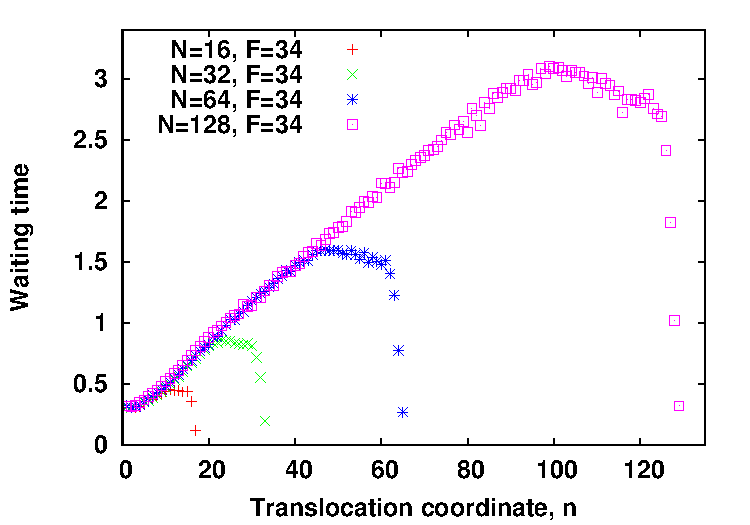
\includegraphics[width=0.9\textwidth]{waitingtime.pdf}


\caption[Temps d'attente des monomères]{Temps d'attente des monomères au cours de la translocation. Le temps d'attente augmente de manière affine jusqu'à atteindre un pallier en fin de translocation. Le début de la translocation est, à force constante, identique quelque soit la longueur du polymère. La translocation est alors caractérisée par trois phases. Lors de la première phase, le temps d'attente des monomères augmente de façon affine. la deuxième phase est caractérisée par un plateau du temps d'attente. la dernière phase correspond à une chute du temps d'attente, c'est la rétractation de la queue du polymère en fin de translocation et ne semble pas dépendre de N. Le temps de translocation du polymère correspond à l'aire sous la courbe du temps d'attente.}
\label{waitingtime}
\end{center}
\end{figure}


A notre connaissance, l'analyse de ces temps d'attente n'a pas été abordée dans la littérature. Nous nous proposons d'élaborer un modèle qui va décrire la physique de la translocation et expliquer l'origine des effets de taille finie qui font sous-estimer $\alpha$. Nous allons proposer une évolution polynomiale du temps de translocation sous la forme $aN +b N^2$, les effets de taille finie étant inclus dans le premier degré du polynôme. La superposition des temps d'attente en début de translocation (voir figure \ref{waitingtime}), quelque soit la taille du polymère sera la base de notre raisonnement. Le réajustement de ces temps d'attente, présenté sur la figure \ref{waitingtimerescaled}, a aiguillé notre réflexion.


\begin{figure}[H]
\begin{center}
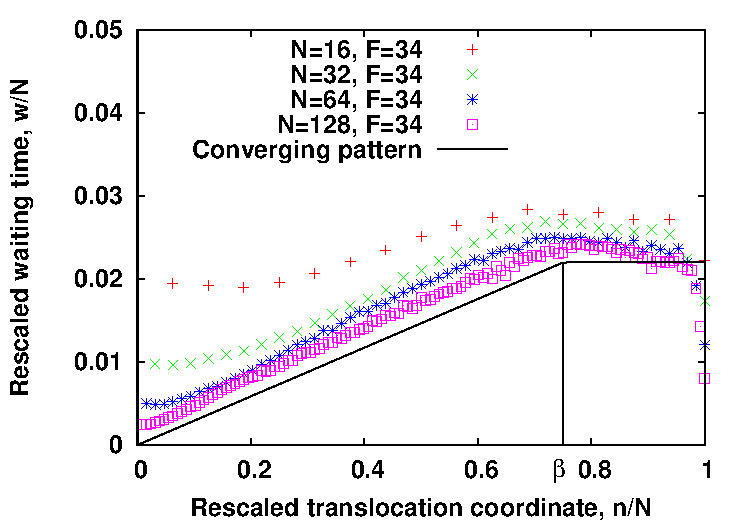
\includegraphics[width=0.9\textwidth]{waitingtimerescaled.pdf}


\caption[Réajustement des temps d'attente des monomères]{Réajustement des temps d'attente des monomères au cours de la translocation. Lorsque la chaîne est longue, la première phase tend à être de plus en plus proche d'une fonction linéaire, le début de la seconde phase semble, à une force donnée, apparaître à une fraction fixe du polymère $\beta$. La deuxième phase semble montrer que les plateaux convergent a un temps d'attente proportionnel à $N$. La dernière phase est négligeable sur le temps de translocation. L'aire totale sous la courbe réajusté converge vers un triangle de accolé à un rectangle. Cette convergence vers une aire réajustée constante suggère un comportement de $\tau$ qui converge vers $\tau \propto N^{\alpha}$ avec $\alpha=2$.}
\label{waitingtimerescaled}
\end{center}
\end{figure}


Nous nous sommes demandé ce qui va induire l'apparition du palier dans le temps d'attente des monomères. Nous nous proposons de considérer notre système en regardant séparément la partie transloquée du côté trans de la partie toujours du côté cis. Le pore sépare effectivement ces deux parties. Déterminons des échelles de vitesse caractéristiques de chacune des parties. Pour le côté trans, le système est dominé par la force qui le tracte depuis le bout de la chaîne, l'échelle de vitesse associée au niveau de la membrane, lorsque $n$ monomères sont du côté trans, est :

\begin{center}
\begin{eqnarray}
v^*_{trans} \propto \frac{f}{\nu n}
% f_{trans}^*\propto \frac{f}{n}
\end{eqnarray}
\end{center}

Du côté cis, toujours à l'équilibre, la diffusion brownienne dont la racine carré de la force quadratique moyenne associée, divisée par le coefficient de frottement va donner l'échelle de vitesse caractéristique:

\begin{center}
\begin{eqnarray}
v^*_{cis} \propto \frac{\sqrt{\nu(N-n)k_BT}}{\nu(N-n)} = \sqrt{\frac{k_BT}{\nu(N-n)}}
%f_{cis}^*\propto \sqrt{\frac{k_BT}{\nu(N-n)}}
\end{eqnarray}
\end{center}

On s'attend a un changement de comportement lorsque la vitesse caractéristique du côté trans ne domine plus celle du côté cis. En effet, l'observation de l'évolution de la coordonnée de translocation (le nombre de monomère ayant effectué la translocation) présentée sur la figure \ref{transloccoordinate} permet d'observer deux régimes différents.


\begin{figure}[H]
\begin{center}
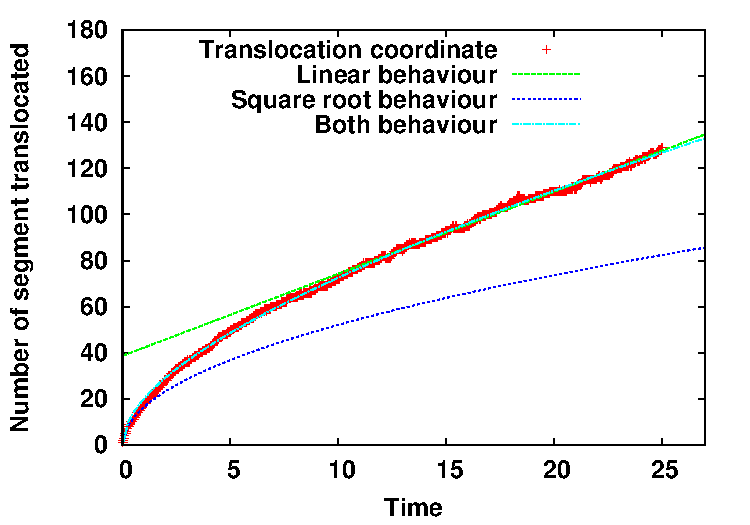
\includegraphics[width=0.9\textwidth]{transloccoordinate.pdf}
\caption[Fluctuations de la coordonnée de translocation]{Evolution de la coordonnées de translocation d'un polymère de taille N=128 tracté à force f=34. En début de translocation, l'évolution du nombre de monomère ayant effectué la translocation est monotone et évolue en $\sqrt{t}$, puis l'évolution devient linéaire avec des fluctuations qui suggèrent une diffusion biaisée avec des fluctuations d'origines thermiques plus grandes que le biais. Nous somme ici dans le cas N=128, ce qui nous permet d'avoir un comportement initial  qui s’affranchit des effets de taille finie.}
\label{transloccoordinate}
\end{center}
\end{figure}

 Dans le premier régime, la coordonnée de translocation ($n$) évolue proportionnellement à $\sqrt{t}$, ce qui est pertinent si l'on considère la prédominance d'une échelle de force inversement proportionnelle à $n$, car l'échelle de vitesse correspondante est également inversement proportion- nelle à $n$, ce qui entraîne une augmentation linéaire du temps d'attente. Pour le deuxième régime, l'évolution affine de la coordonnée de réaction est en accord avec une vitesse de translocation constante (donc un temps d'attente constant également). Les fluctuations traduites par la non monotonie de $n(t)$ (i.e. Le retour possible de monomères du côté trans) suggèrent la prédominance d'un processus de diffusion biaisée.


Comparons donc les échelles proposées:

\begin{center}
\begin{eqnarray}
v^*_{trans}\approx v^*_{cis}
\end{eqnarray}
\end{center}

%\begin{center}
%\begin{eqnarray}
%f^*_{trans}\approx f^*_{cis}
%\end{eqnarray}
%\end{center}
%
%\begin{center}
%\begin{eqnarray}
%f^*_{trans}\approx f^*_{cis}
%\end{eqnarray}
%\end{center}

\begin{gather}
\frac{f}{\nu n} \propto  \sqrt{\frac{k_BT}{\nu(N-n)}} \\
\frac{f^2}{n^2} \propto \frac{\nu k_BT}{(N-n)}
\label{propscale}
\end{gather}
Introduisons le paramètre C, qui défini le lien de proportionnalité de l'équation précédente \ref{propscale}.
\begin{gather}
\frac{f^2}{n^2} = \frac{C}{(N-n)}\\
n^2C^2 +f^2n-f^2N=0
\label{equsnddegre}
\end{gather}
La valeur seuil de n à partir de laquelle le temps d'attente des monomères atteint un palier est la racine positive de l'équation du second degré précédente \ref{equsnddegre}.
\begin{center}
\begin{eqnarray}
n_{seuil}=\frac{f^2(\sqrt{1+(4NC/f^2)}-1)}{2C}
\label{nseuil}
\end{eqnarray}
\end{center}
Lorsque $f \gg \sqrt{CN}$, c'est à dire lorsque l'échelle de force de la traction est dominante du côté trans pendant toute la translocation, $n_{seuil} \rightarrow N$, la phase comportant un temps d'attente linéaire dure l'intégralité de la translocation. Nous avons observé que la fraction du polymère à partir de laquelle le changement de régime a lieu, $\beta(f,N)=n_{seuil}/N$ dépend uniquement de la variable A:

\begin{center}
\begin{eqnarray}
A= \frac{2CN}{f^2}
\end{eqnarray}
\end{center}
alors,
\begin{center}
\begin{eqnarray}
\beta(f,N)= \frac{n_{seuil}}{N}= \beta(A)= \frac{\sqrt{1+2A}-1}{A}
\end{eqnarray}
\end{center}
%Dérivons cette expression par rapport à N
%\begin{center}
%\begin{eqnarray}
%\frac{\partial\beta(f,N)}{\partial N}= \frac{\partial\beta(A)}{\partial A}\frac{\partial A}{\partial N}= \frac{A}{N}\beta'(A)
%\end{eqnarray}
%\end{center}
%avec $\beta'(A)$:
%\begin{center}
%\begin{eqnarray}
%\beta'(A)=  \frac{1}{\sqrt{A+2A^2}}-\frac{\sqrt{1+2A}-1}{A^2} \rightarrow A\cdot \beta'(A)=  \frac{1}{\sqrt{1+2A}}-\frac{\sqrt{1+2A}-1}{A}
%\end{eqnarray}
%\end{center}
%Vérifions les limites de $A \cdot \beta'(A)$ 
%\begin{center}
%\begin{eqnarray}
%\lim\limits_{A \rightarrow +\infty}\left(A \cdot \beta'(A)\right)= \lim\limits_{A \rightarrow +\infty}\left(\frac{1}{\sqrt{1+2A}}\right)-\lim\limits_{A \rightarrow +\infty}\left(\frac{\sqrt{1+2A}-1}{A}\right)=0
%\end{eqnarray}
%\end{center}
%
%\begin{gather}
%\lim\limits_{A \rightarrow 0}(A \cdot \beta'(A))= \lim\limits_{A \rightarrow 0}\left(\frac{1}{\sqrt{1+2A}}-\frac{\sqrt{1+2A}-1}{A}\right)\nonumber \\
%= \lim\limits_{A \rightarrow +0}(1 + 2A - 1 + \frac{1}{8}A + o(A^2) )= 0
%\end{gather}
%La fonction $A \rightarrow A \cdot \beta'(A)$ est définie, continue et dérivable sur $\mathds{R}^{+}$ avec des limites aux bornes finies, elle est donc bornée. Ce qui signifie que:
%
%
%\begin{center}
%\begin{eqnarray}
%\lim\limits_{N \rightarrow +\infty}\left(\frac{\partial\beta(f,N)}{\partial N}\right)= \lim\limits_{N \rightarrow +\infty}\left(\frac{A}{N}\beta'(A)\right)=0
%\end{eqnarray}
%\end{center}
%
%C'est à dire que pour $N$ suffisamment, la fraction du polymère à laquelle le changement de régime a lieu ne dépend que de la valeur de $f$.  
%
%De même, 
%
%\begin{gather}
%\frac{\partial\beta(f,N)}{\partial f}= \frac{\partial\beta(A)}{\partial A}\frac{\partial A}{\partial f}= \frac{-2A}{f}\beta'(A) \\
%\Rightarrow\lim\limits_{f \rightarrow +\infty}\left(\frac{\partial\beta(f,N)}{\partial f}\right)= \lim\limits_{f \rightarrow +\infty}\left(\frac{-2A}{f}\beta'(A)\right)=0
%\end{gather}
%
%Ce dernier résultat permet de dire que pour $f$ et $N$ suffisamment grand, $\beta$ ne dépend plus que de $A=\frac{2CN}{f^2}$ et reste relativement stable.





L'analyse des temps d'attente n'ayant pas été initialement prévue dans nos simulations, nous avons choisi un polymère plutôt court de 32 grains pour tester l'évolution de $\beta$,  malgré les forts effets de taille finie. En travaillant à taille constante, nous avons vérifié que l'aire sous la courbe des temps d'attente reste approximativement constante (voir \ref{verifbetawaitingtimesamen}) et converge également vers une aire réajustée en force constante.

\newpage

\begin{figure}[H]
\begin{center}
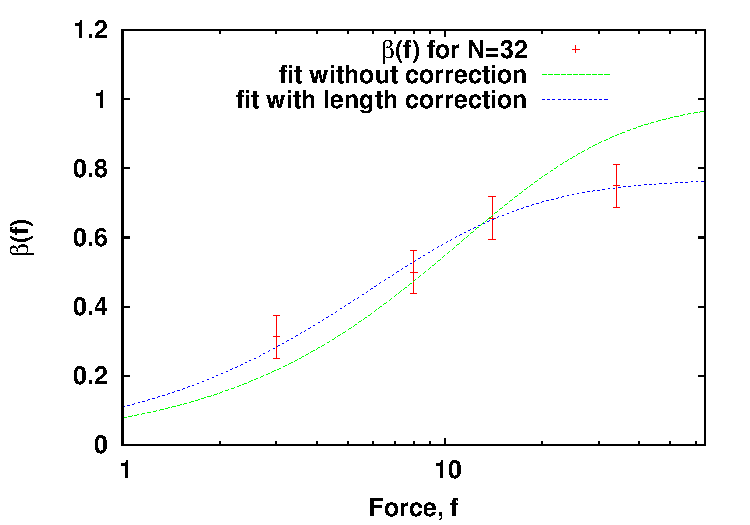
\includegraphics[width=0.85\textwidth]{betaf.pdf}
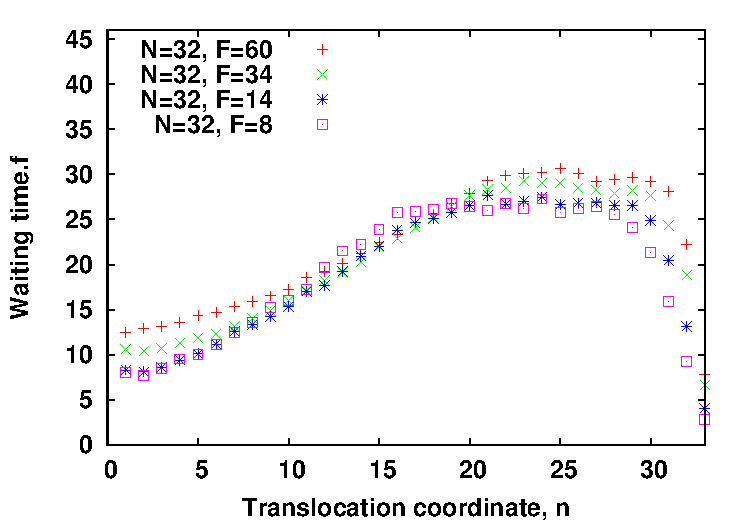
\includegraphics[width=0.85\textwidth]{waitingtimen32foisf.pdf}


\caption[Plateau des temps d'attente et comportement en fonction de la force]{En haut: Vérification du plateau des temps d'attente pour un polymère de taille N=32 à diverses valeurs de forces. La formule que nous avons établi fitte mieux avec une valeur de N effective plus faible $N_{eff} =28$, ce qui correspond aux 4 monomères pour lesquels le temps d'attente est en chute forte, il s'agirait donc de forts effets de taille finie (on a alors $\beta$ qui ne tend pas vers 1 mais vers 28/32). On est toujours dans le régime ou $\beta$ dépend de $f$. A partir de $f>10$, $\beta$ ne varie que très peu et peut être considéré comme constant sur plus d'un ordre de grandeur. En bas: L'aire sous la courbe du temps d'attente des monomères semble être proportionnelle à la force exercée. Pour f=60, on est dans le cas de liaisons étirées où $\delta=0.8$. L'ordonnée à l'origine semble dépendre linéairement de $f$ tant que la force ne permet pas d'étendre les liaisons. $\beta$ n'évolue que faiblement lorsque la force devient suffisamment grande. On convergerait également vers une aire réajustée constante si les liaisons n'étaient pas extensibles.}
\label{verifbetawaitingtimesamen}
\end{center}
\end{figure}



Le temps d'attente ayant en première partie un comportement affine, appelons D l'ordonnée à l'origine et B le coefficient de la pente en première phase. On peut alors déduire le temps de translocation en intégrant le temps d'attente des monomères.


\begin{center}
\begin{eqnarray}
\tau(f,N) = \int_0^N w(n) dn = \int_0^N D(f) dn + \int_0^{\beta N} B(f) n \cdot dn + \int_{\beta N}^{N} \beta\cdot B(f) N dn  
\end{eqnarray}
\end{center}

 B est linéaire en force, donc $B=\frac{B'}{f}$. En supposant comme le suggère la figure \ref{verifbetawaitingtimesamen} que les effets de taille finie sont également linéaires en force, ce qui signifie que  $D=\frac{D'}{f}$, on obtient l'expression suivante:
 
\begin{center}
\begin{eqnarray}
\tau(f,N) = \frac{D'}{f} N + \frac{B' \cdot \beta(A)^2}{2f}N^2 +(1-\beta(A)) \cdot \frac{\beta(A) B'}{f}N^2
\end{eqnarray}
\end{center}
\begin{center}
\begin{eqnarray}
\boxed{\tau(f,N) = \frac{D'}{f} N + (\beta(A)-\frac{\beta(A)^2}{2}) \frac{B'N^2}{f}}
\label{tauformula}
\end{eqnarray}
\end{center}

 Pour des valeurs de force raisonnables, c'est à dire $A<1$, le pré-facteur devant le terme en $\frac{N^2}{f}$ est quasiment constant, comme le montre la figure \ref{timebeta}. 

\begin{figure}[H]
\begin{center}
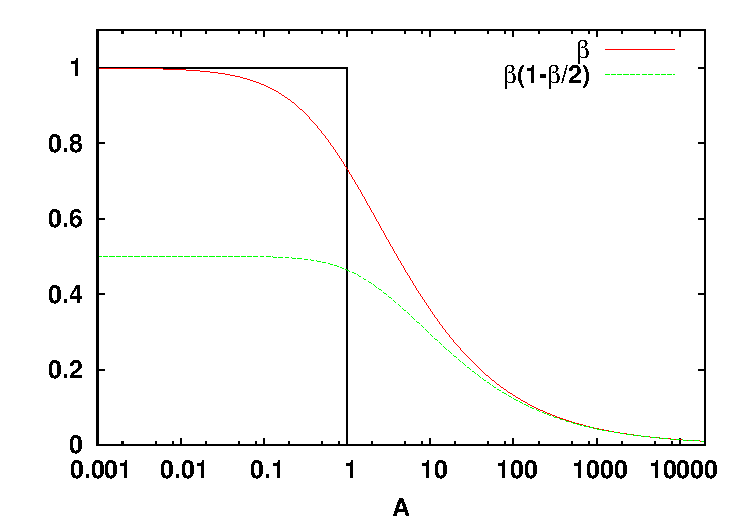
\includegraphics[width=0.85\textwidth]{timebeta.pdf}

\caption[Préfacteur du temps de translocation]{Dépendance de la fraction à laquelle a lieu le changement de régime et du pré-facteur devant le terme en $\frac{N^2}{f}$ dans le calcul du temps de translocation en fonction de $A= \frac{2CN}{f^2}$. Pour des valeurs de A inférieures à 1, le pré-facteur est quasiment constant. Cette condition semble réalisée lorsque la probabilité d'effectuer la translocation est proche de 1.}
\label{timebeta}
\end{center}
\end{figure}

Lorsque la probabilité d'effectuer la translocation est suffisamment élevée, nous nous situons dans la plage encadrée sur la figure \ref{timebeta} et donc les variations du pré-facteur de l'équation \ref{tauformula} sont négligeables. Testons donc cette dernière équation.



\begin{figure}[H]
\begin{center}
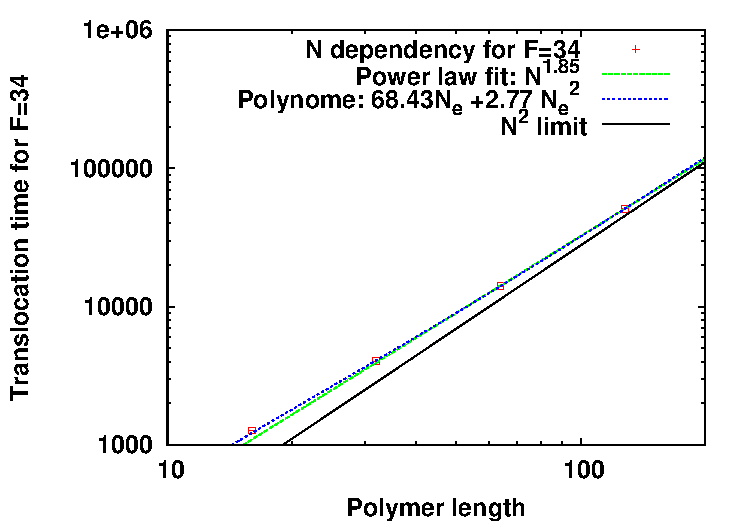
\includegraphics[width=0.9\textwidth]{ndeppolsimplef34.pdf}

\caption[Comparaison polynôme et loi de puissance]{Comparaison de l'évaluation du temps de translocation par une loi de puissance et par un polynôme de degré 2. Notre proposition d'un polynôme de degré deux sans terme constant avec une taille effective $N_e = N-4$ correspondant à un polymère amputé de la queue qui se rétracte en fin de translocation, évalue mieux le temps de translocation et les effets de taille finis que la loi de puissance simple. Notre modèle prévoit une convergence avec la loi de puissance tel que $\alpha=1.99$ pour N=2315.}
\label{verifpol}
\end{center}
\end{figure}

En utilisant une valeur efficace $N_e=N-4$ correspondant à la suppression de 4 monomères suite à la rétractation de la queue, nous obtenons une très bonne évaluation du temps de translocation.

\newpage

\subsection{Translocation du polymère structuré, pore large}

Nous venons de vérifier des propriétés déjà présentées et faisant consensus dans la littérature, et avons également apporté notre contribution théorique à l'explication du processus de translocation par une force exercée en bout de chaîne. Cette base solide va maintenant nous permettre d'étudier le cas d'un polymère structuré. Etudions donc la translocation de notre polymère structuré à travers un pore large également.\\

Nous utilisons cette fois ci le pore plus large présenté précédemment (figure \ref{bothpores}). On a alors une configuration dont les propriétés sont présentées dans la figure \ref{porelarge}. Trois polymères ont été étudiés, ils présentent N= 8, 16 et 32 grains latéraux soit des longueurs de cha\^ine de 16, 32 et 64 grains respectivement, comparables à l'analyse précédente du polymère linéaire. La figure \ref{holebiggertau} présente les temps de translocation moyens en fonction de la force appliquée au polymère ainsi que ces mêmes temps de translocation réajustés.

\begin{figure}[H]
\begin{center}
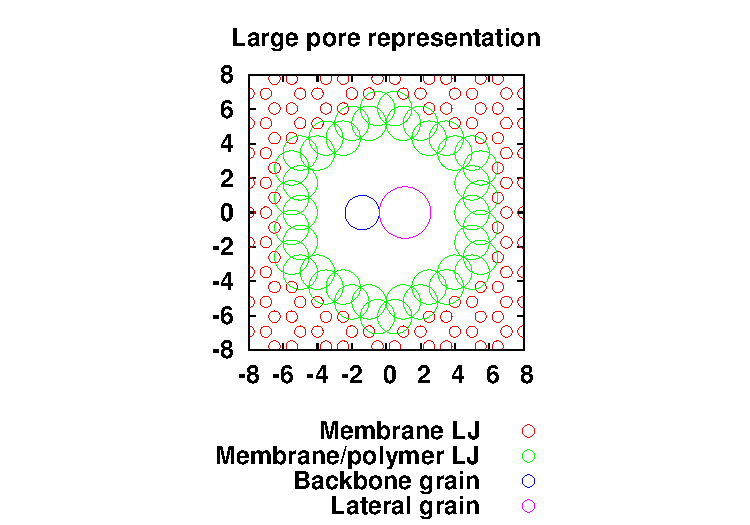
\includegraphics[width=1\textwidth]{largepore.pdf}


\caption[Polymère structuré et pore large]{Pore large utilisé pour la translocation de notre polymère structuré. Les tailles des différents grains sont respectées. }
\label{porelarge}
\end{center}
\end{figure}



\begin{figure}[H]
\begin{center}
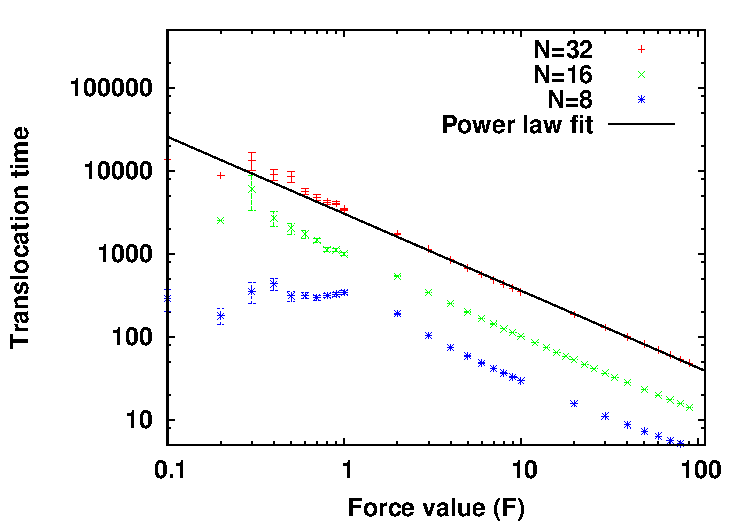
\includegraphics[width=0.9\textwidth]{translocholebigger.pdf} 
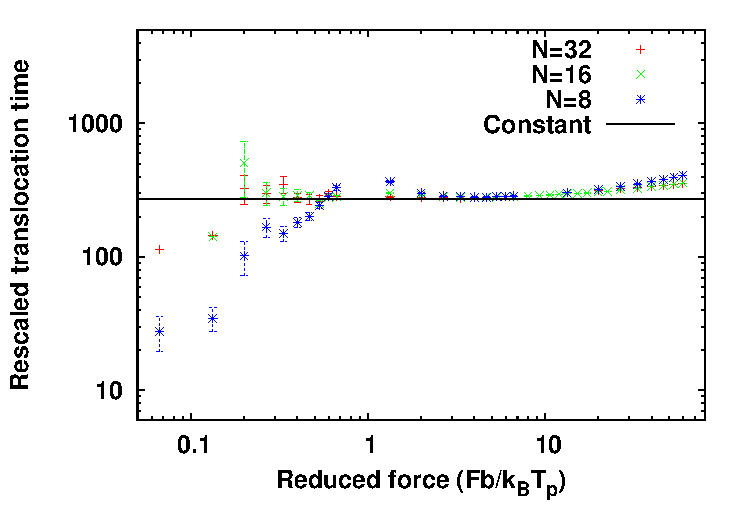
\includegraphics[width=0.9\textwidth]{transloctaufrescholebigger.pdf} 
\caption[Temps de translocations du polymère structuré avec un pore large]{En haut: Temps de translocation moyen du polymère en fonction de la force de traction exercée. Le plateau du cas non biaisé est clair dans le cas N=8, moins pour les autres. En bas: Temps de translocation réajusté (avec la même valeur de $\alpha=1.84$ que précédemment et en prenant une longueur de chaîne de 2N) pour le polymère structuré tiré à travers un pore large. Pour le polymère le plus court, deux régimes clairement distincts sont observables avec une transition de $\delta=0$ à $\delta=1$. On observe cette fois encore une diminution de $\delta$ pour les forces importantes. La constante tracée ici vaut exactement 1.5 fois celle tracée pour le polymère simple. On a donc un temps de translocation 1.5 fois supérieur à cause du grain latéral ajouté pour un grain de la chaîne sur deux.}
\label{holebiggertau}
\end{center}
\end{figure}

La figure \ref{holebiggertau} montre que dans le cas du polymère structuré tiré à travers un pore large, les résultats sont similaires au cas du polymère linéaire simple. La zone pallier où $\delta=0$ n'est clairement visible que dans le cas $N=8$, ce qui se comprend car ce régime n'est pas favorisé par l'ajout de grains latéraux qui ralentissent la diffusion (on a $\frac{1}{2}$ grain supplémentaire par grain du squelette du polymère, ce qui fait un coefficient de friction 1.5 fois supérieur à longueur de chaîne égale). On observe toujours deux régimes, l'un proche de la translocation non biaisée, l'autre proche de $\alpha= 1.81$ et $\delta=1$ lorsque la translocation est pilotée par la chaîne étirée du côté trans. Les paramètres de friction et de force des liaisons, comme dans le cas précédent expliquent une diminution de $\delta$ à fortes forces.

Les distributions des temps de translocation sont encore une fois similaires au cas précédent. Nous avons extrait, à l'aide du même type d'analyse, les vitesses de biais associées à la diffusion du pore le long du polymère. Les résultats sont présentés et comparés au cas du polymère linéaire simple sur la figure \ref{frictionholebigger}.


\begin{figure}[H]
\begin{center}

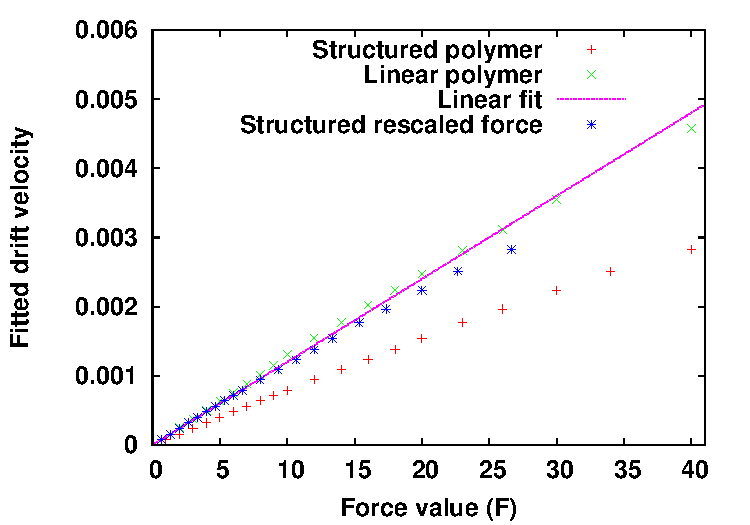
\includegraphics[width=0.9\textwidth]{largeporesfirction.pdf}

\caption[Friction et translocation pour polymère structuré avec un pore large]{Estimation du coefficient de la vitesse de diffusion du pore le long du polymère. Nous avons estimé la vitesse de biais de la diffusion du pore dans le cas du polymère structuré et la comparons au cas précédent pour une même longueur de chaîne de 32 grains. On peut voir que notre cas est équivalent au précédent si on divise la force appliquée en bout de chaîne par 1.5, ce qui équivaut à un coefficient de frottement $\xi$ qui est 1.5 fois plus élevé, ce qui correspond bien à la présence de 1.5 fois plus de grains dans le système.}
\label{frictionholebigger}
\end{center}
\end{figure}

La seule différence concrète est donc une vitesse de translocation moindre, à cause du coefficient de friction augmenté par la multiplication du nombre de grains par 1.5.


Afin de ralentir la translocation, enjeu clé du séquençage, nous allons maintenant étudier l'influence d'un nanopore plus étroit. En quoi le frottement important induit par le pore va-t-il modifier les lois d'échelle trouvées précédemment ?






%A l'instar des prédictions de J. L. A. Dubbeldam et collaborateurs \cite{Dubbeldam2012}, nous observons deux régimes distincts caractérisant la dépendance de la loi d'échelle avec la force. En effet, on observe à forces faibles (excepté pour $N=8$) et intermédiaires un comportement tel que $\tau \propto 1/F$. Pour des forces plus élevées, on trouve une loi d'échelle avec un exposant plus élevé ($\tau \propto F^{-0.74}$ pour N=8) Cet exposant plus élevé montre la transition vers $\tau \propto F^{(1/\nu) -2}$. La valeur plus faible qu'attendue peut être attribuée aux effets de taille finie et à l'amplitude de la force qui n'est pas assez élevée. De plus la transition entre les régime semble apparaitre plus tôt pour les $N$ faibles, contrairement à la prédiction de J. L. A. Dubbeldam et collaborateurs \cite{traction}. Cette différence pourrait venir du fait que nous tractons notre polymère (force en bout de chaîne), alors que dans leur cas, une différence de potentiel est appliquée (force au sein du pore). La Figure \ref{holebigger} permet de mieux visualiser ces régimes. En ce qui concerne l'évolution de $\tau$ avec $N$, on trouve un exposant de 1.78 pour les forces imposées de 9 et 20, et 1.69 pour 80. Ces valeurs sont proches du cas $\tau \propto N^{(1+\nu)}$ attendu pour les forces importantes.
%
%Dans le cas $N=8$, nous observons un décrochement de pente. Ceci se produit lorsque la force est faible et pour une chaîne très courte. L'impulsion initiale donnée par le mouvement brownien rejette nombre de configurations (d’où une forte diminution du nombre de translocation réussies), celles conservées ayant une grande impulsion non naturelle dans le sens de la translocation, diminuant artificiellement $\tau$. Cette rupture de pente nous semble donc être un effet de taille finie.



\subsection{Translocation du polymère structuré, pore étroit}


Nous étudions dorénavant l'effet d'une membrane fixe munie d'un nanopore étroit qui va induire un frottement plus important. Le nanopore est créé en supprimant uniquement 24 grains au centre cette fois ci (voir figure \ref{porethin}). Le pore a été choisi suffisamment étroit pour limiter le passage des monomères de front, ils devront se déformer pour permettre au grain latéral, plus volumineux, d'effectuer la translocation.

\begin{figure}[H]
\begin{center}
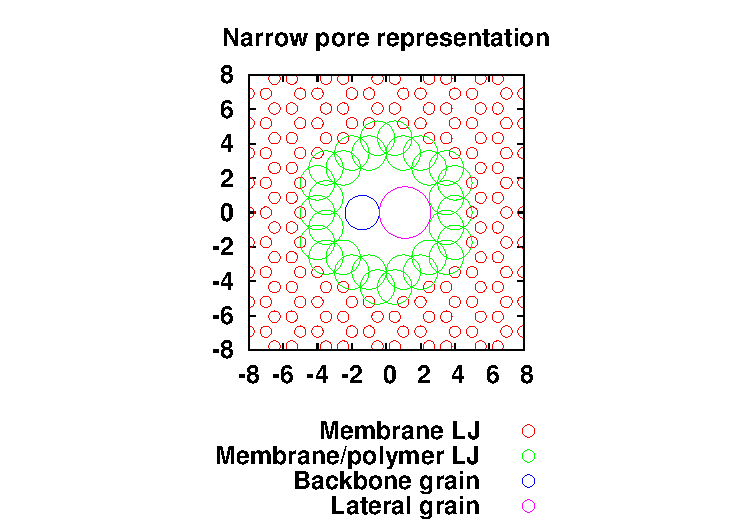
\includegraphics[width=1\textwidth]{thinpore.pdf}


\caption[Polymère structuré et pore étroit]{Pore étroit utilisé pour la translocation de notre polymère structuré. Les tailles des différents grains sont respectées. Le diamètre du pore a été choisi suffisamment étroit pour multiplier les contacts avec ce dernier. La liaison entre la chaîne du polymère et les grains latéraux permettent une déformation pour traverser le pore.}
\label{porethin}

\end{center}
\end{figure}

La figure \ref{sptransloc} montre l'évolution des temps de translocation sur une plage de force privée de sa partie inférieure, faute de statistiques suffisantes. Les résultats sont également comparés au cas du pore large.

\begin{figure}[H]
\begin{center}
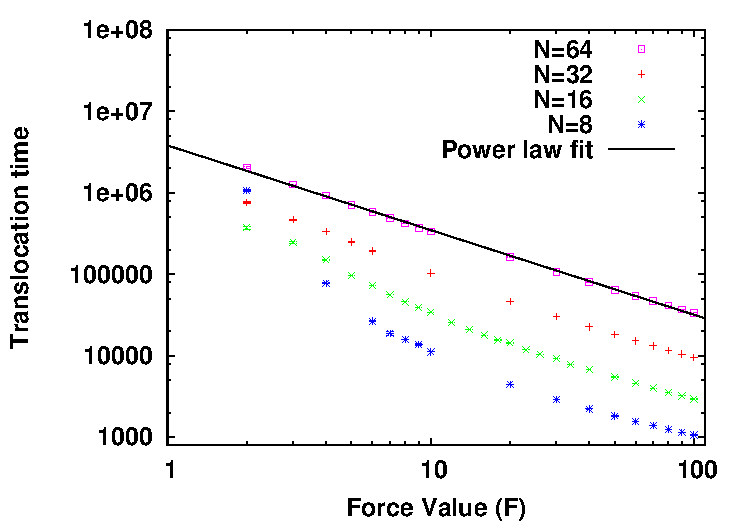
\includegraphics[width=0.9\textwidth]{sptransloc.pdf}

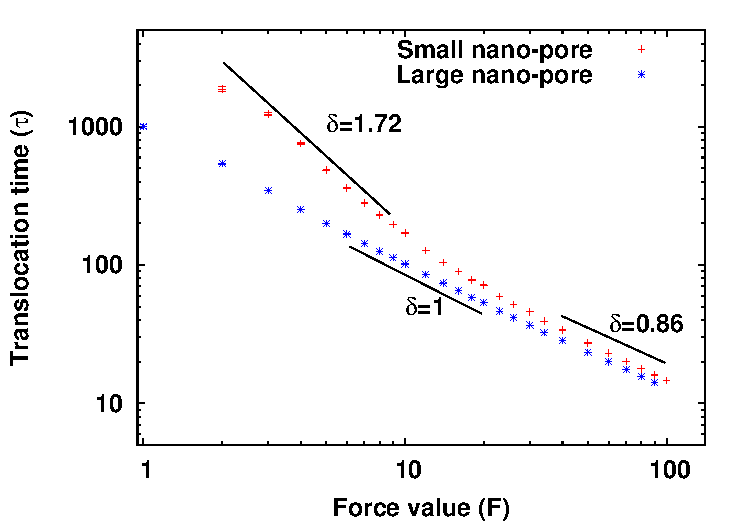
\includegraphics[width=0.9\textwidth]{complargenarrowtransloc.pdf} 
\caption[Temps de translocations du polymère structuré, comparaison]{Temps de translocation du polymère structuré à travers un pore étroit et comparaison avec le pore large. Par rapport au cas du pore large, le spectre des forces balayé est amputé d'une décade. En effet, les translocation menées à bien ne sont statistiquement significatives que pour $f>1$.}
\label{sptransloc}
\end{center}
\end{figure}


A fortes forces, les données sont très proches du cas du pore large, il y a convergence entre les deux systèmes. Dans le cas de forces faibles en revanche, les deux systèmes sont très différents. Pour des forces trop faibles, inférieures à l'ordre de l'unité, les translocation n'aboutissent plus. Le polymère sort quasi systématiquement du côté cis. Pour les forces intermédiaires, la translocation est fortement ralentie, elle est jusqu'à un ordre de grandeur plus lente. Quelle est l'influence de ses changements radicaux sur les exposants critiques $\alpha$ et $\delta$ ? Avons nous toujours 2 régimes ? Nous tâchons d'éclaircir ces questions dans à l'aide de la figure \ref{sptransloctaufresc} qui présente les temps de translocation réajustés.


\begin{figure}[H]
\begin{center}
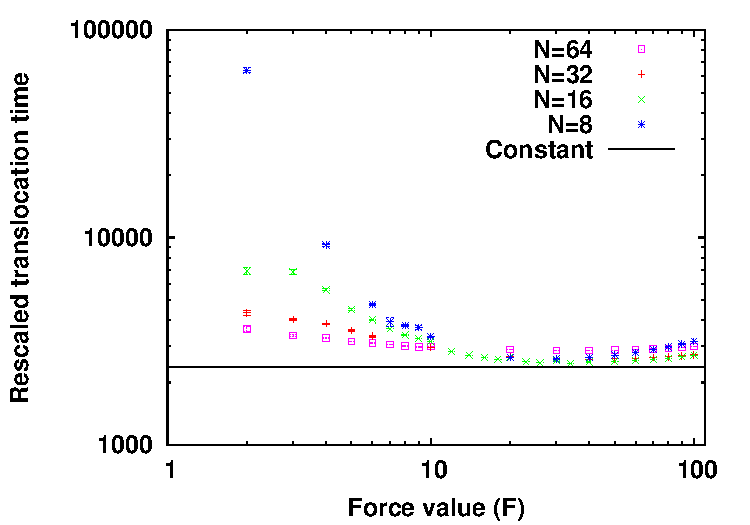
\includegraphics[width=0.9\textwidth]{sptransloctaufresc.pdf}
\caption[Temps de translocations réajustés (avec $\alpha=1.73$) du polymère structuré et pore étroit]{Temps de translocation réajusté du polymère dans le cas d'un nanopore étroit. A forces importantes, comme nous l'avions soupçonné, rien ne change, on observe toujours une transition de $\delta=1$ vers une valeur plus faible à cause de la faiblesse des liaisons et/ou de la friction avec le solvant trop importante. Dans le cas des forces modérément faibles, nos résultats sont inédits, avec $\delta>1$. La statistique de ses points devient de plus en plus faible à mesure que l'on approche de la valeur de force $f=1$.}
\label{sptransloctaufresc}
\end{center}
\end{figure}

Afin de comprendre ce comportement différent à faibles forces, nous nous sommes intéressés aux différences entre les pores concernant la probabilité de translocation et la vitesse moyenne de biais estimée avec les distributions du temps de translocation. Les résultats obtenus, présentés sur la figure \ref{compporesizeprobafriction}, nous font suggérer l'apparition d'une force seuil nécessaire à l'accomplissement de la translocation. Nous avons montré précédemment que la vitesse de translocation était linéaire en force, ce qui nous amène a penser que le pore étroit induit des frottements supplémentaires tels que la vitesse moyenne de translocation s'exprime selon:

\begin{center}
\begin{eqnarray}
v_{moy}=\frac{f- f_s}{\nu N}
\end{eqnarray}
\end{center}



\begin{figure}[H]
\begin{center}
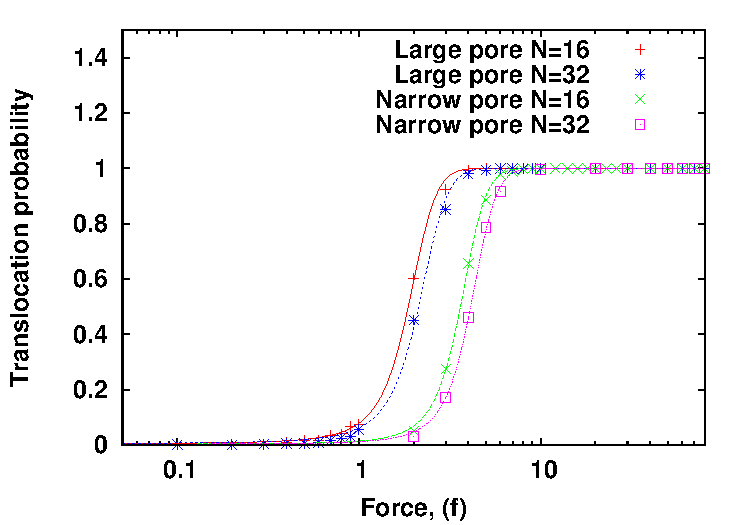
\includegraphics[width=0.9\textwidth]{probatransloccomppores.pdf} 
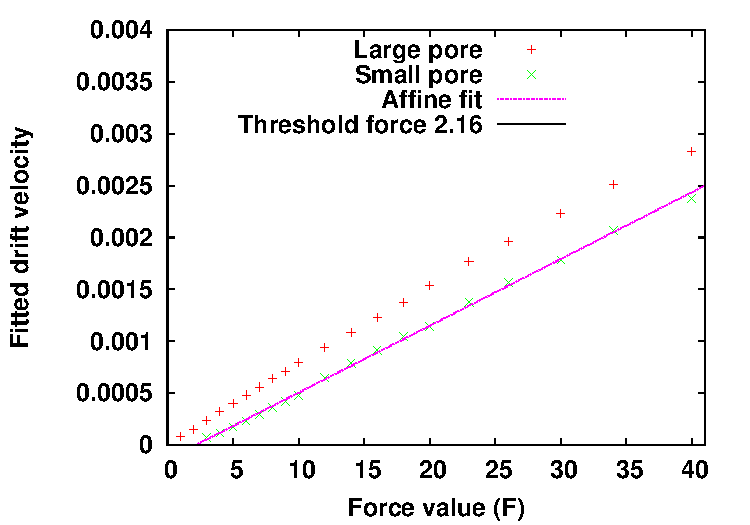
\includegraphics[width=0.9\textwidth]{structuredporesfirction.pdf} 
\caption[Différences de friction et de probabilité de translocations entre les pores]{En haut: Comparaison de la probabilité de translocation entre les deux nanopores. L'étroitesse du pore entraîne une augmentation de la force nécessaire pour avoir une probabilité de translocation égale à 0.5, pour un polymère de taille N=16, cela représente une différence de force de 1.75. En bas: estimation de la vitesse de biais obtenue à partir des distributions de temps de translocation. On observe une évolution non plus linéaire mais affine, de même pente mais avec une ordonnée à l’origine différente, ce qui équivaut à l'application d'une force effective $f_e=(f-f_s)$ réduite avec une force seuil $f_s =2.16$, estimée lorsque la valeur de la vitesse de biais devient nulle.}
\label{compporesizeprobafriction}
\end{center}
\end{figure}

Nous calculons cette force seuil de deux manières différentes, avec la probabilité de translocation du côté trans et avec la friction extraite de l'analyse de la distribution des temps de translocation (voir figure \ref{compporesizeprobafriction}). Les deux valeurs extraites sont comparables (1.75 et 2.17) et correspondent effectivement au moment ou la translocation avorte dans la majorité des cas car le polymère reste du côté cis de la membrane. La valeur $\delta=1.75$ trouvée pour les faibles forces dans le cas N=16 n'est pas universelle car elle ne s'applique pas aux autres longueurs de chaînes. Aucune valeur de $\alpha$ pertinente ne peut être estimée non plus.\\

Bien que le cas du pore étroit ne soit pas entièrement élucidé à faibles forces, c'est le pore que nous allons conserver pour la partie suivante, afin d'étudier les propriétés de la membrane, car c'est le pore qui va maximiser les interactions polymère membrane.


%
%Encore une fois, nous observons les deux régimes précédents. Cependant la frontière semble apparaitre plus tard à cause du frottement, ce qui diminue la force effective appliquée sur le polymère ($F_{eff}=F-\epsilon _{pore})$. Les mêmes lois d'échelles sont observées à forte force ( $\tau \propto 1/F$ puis $\tau \propto F^{(1/\nu) -2}$).\\
%
% Une grande différence s'observe dans le cas de l'application de forces faibles. Comme la Figure \ref{thinpore} le suggère, les translocations n'ont pas pu être menées à bien pour des forces inférieures à l'unité.
%
%Les contraintes stériques choisies entrainent une modification de la barrière d'énergie. La translocation des grains par groupe de trois (1 grain latéral volumineux à la fois), comme nous l'illustrerons dans la section suivante (Figure \ref{temperature}), corrobore une hypothèse de déformation de la barrière entropique en dents de scies décroissante. Cette modification est significative puisqu'elle empêche complétement la translocation si la force appliquée est trop faible, elle semble aussi être responsable du comportement inattendu décrit dans la Figure \ref{thinpore}.
%
%Le cas $N=8$ présente encore une fois des problèmes. Lorsque la force est trop faible, les polymères ne pénètrent pas à travers la membrane. Dans le cas de $N=8$, la force est à peine suffisante pour permettre la translocation et n'est pas prépondérente par rapport au bruit thermique. Le polymère passe alors un temps important à rebondir sur le pore avant d'entamer la translocation. Le temps de translocation est alors fortement surévalué (un point a été conservé sur la Figure \ref{thinpore}, pour illustrer ce problème).
%
%
%
%
%
%Nous allons maintenant nous intéresser à l'influence des propriétés vibrationnelles du graphène sur la translocation.



